\documentclass[10pt]{beamer}
\usepackage{booktabs,siunitx}
\usepackage[default]{opensans}
\usetheme{Madrid}
\usefonttheme{default}
\useinnertheme{circles}
\sisetup{detect-all}
\setbeamertemplate{navigation symbols}{} % Uncomment this line to remove the navigation symbols from the bottom of all slides
\setbeamertemplate{caption}{\raggedright\insertcaption\par}

\title[ITS \& MFT Analysis]{A preliminary analysis of pilot beam data from ALICE's new ITS and MFT detectors} % The short title in the optional parameter appears at the bottom of every slide, the full title in the main parameter is only on the title page

% \subtitle{Optional Subtitle} % Presentation subtitle, remove this command if a subtitle isn't required

\author[Miles Kidson]{Miles Kidson \\[1ex] {\small Supervisors: Prof. Zinhle Buthelezi \and Dr. SV Fortsch \and Prof. Tom Dietel \\ Assisted By Dr. B Naik (Postdoctoral fellow)}} % Presenter name(s), the optional parameter can contain a shortened version to appear on the bottom of every slide, while the main parameter will appear on the title slide

\institute[UCT]{University of Cape Town \\ \smallskip \textit{kdsmil001@myuct.ac.za}} % Your institution, the optional parameter can be used for the institution shorthand and will appear on the bottom of every slide after author names, while the required parameter is used on the title slide and can include your email address or additional information on separate lines

\date[November 2022]{Honour's Research Project \\ 2022} % Presentation date or conference/meeting name, the optional parameter can contain a shortened version to appear on the bottom of every slide, while the required parameter value is output to the title slide

\titlegraphic{
\includegraphics[width=35pt]{Figs/ALICE_logo.png}}
\logo{
\includegraphics[width=20pt]{Figs/ALICE_logo_transparent.png}}

\useoutertheme[subsection=false]{miniframes}

\begin{document}

\frame[plain]{\titlepage}

\section{Background}

\begin{frame}
    \frametitle{ALICE Run 3}

    \begin{columns}[c]
        \begin{column}{0.5\textwidth}
            \begin{figure}[h]
                \begin{center}
                    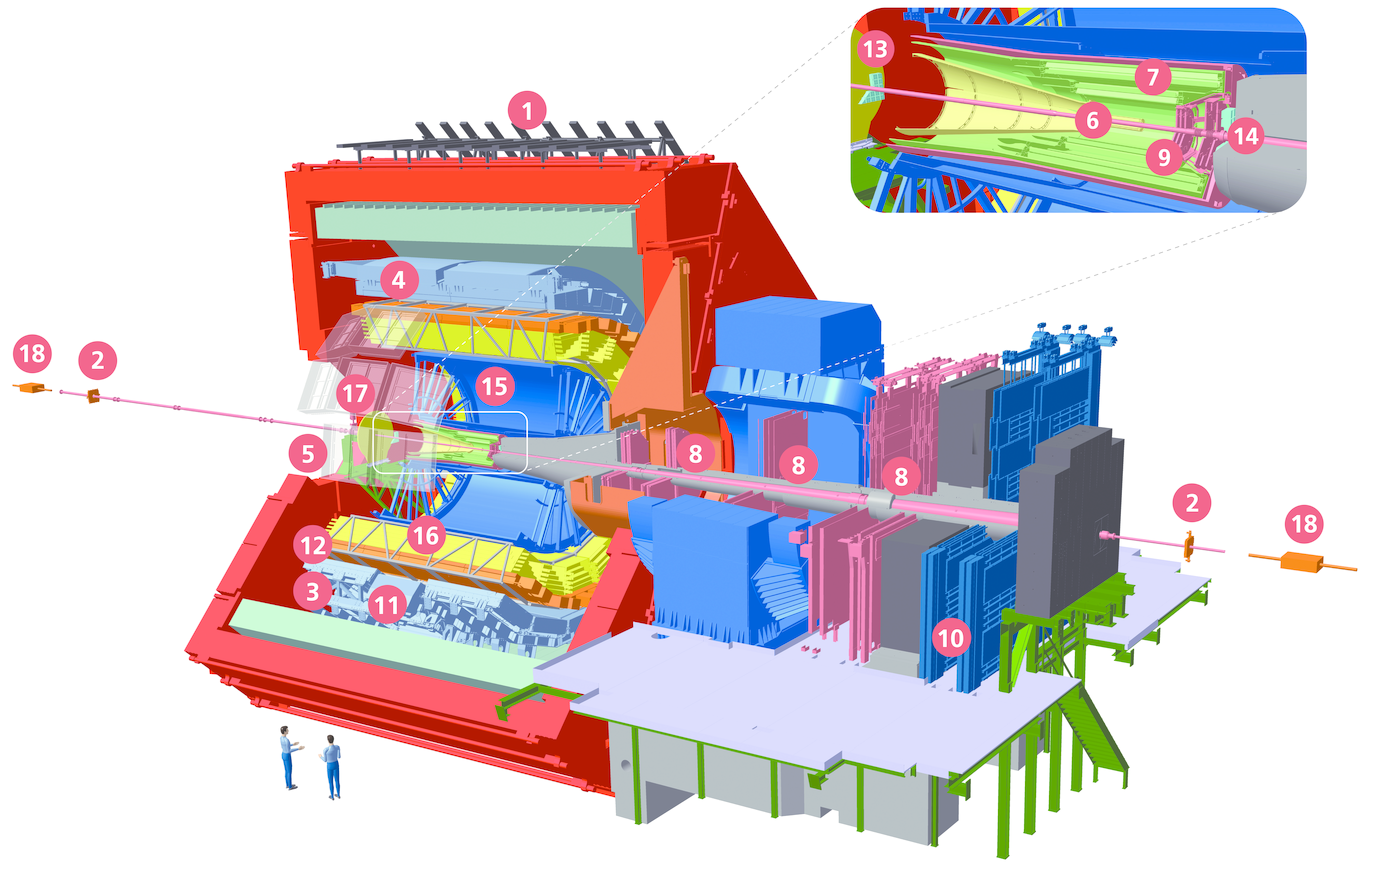
\includegraphics[width=\textwidth]{Figs/ALICE_RUN3_schematic_cropped.png}
                    \caption{ALICE Run 3 Detector Array}
                \end{center}
            \end{figure}
        \end{column}

        \begin{column}{0.5\textwidth}
            \begin{itemize}
                \item LHC Run 3 comes with increased $\sqrt{s}$ and luminosity of collisions
                \item This requires a new untriggered data capture scheme, so detector readout electronics were upgraded at ALICE
                \item The MFT (9) was added, the ITS (6, 7) was upgraded, and the analysis framework was overhauled entirely
                \item Learning this framework, and how the MFT and ITS interact with it, was the main goal of this project
            \end{itemize}
        \end{column}
    \end{columns}

\end{frame}


\begin{frame}
    \frametitle{Coordinate System}

    \begin{columns}[t]
        \begin{column}{0.6\textwidth}
            \begin{itemize}
                \item $Z$: Distance along $Z$-axis (\unit{\centi\metre})
                \item $\varphi$: Azimuthal angle around beam axis
                \item $\theta$: Polar angle
            \end{itemize}
            \begin{figure}[h]
                \begin{center}
                    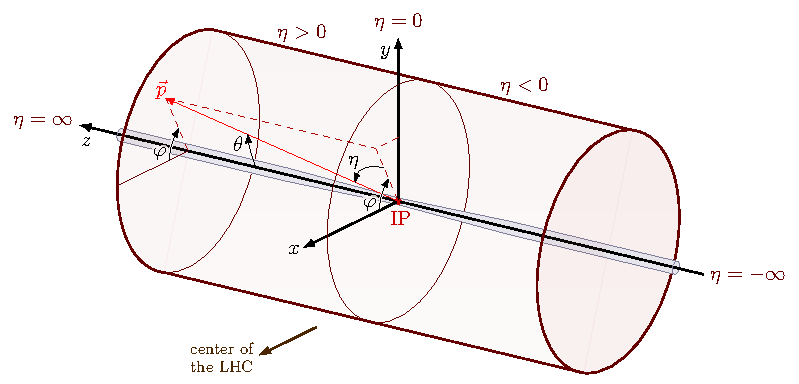
\includegraphics[width=\textwidth]{Figs/coords.pdf}
                \end{center}
            \end{figure}
        \end{column}

        \begin{column}{0.4\textwidth}
            \begin{itemize}
                \item $p_{\mathrm{T}}$: Transverse momentum (\unit{\giga\electronvolt\per c})
                \begin{equation*}
                    p_{\mathrm{T}}=\sqrt{p_x^2+p_y^2}
                \end{equation*}
                \item $y$: Rapidity
                \begin{equation*}
                    y=\frac{1}{2}\ln \frac{E+p_z}{E-p_z}
                \end{equation*}
                \item $\eta$: Pseudorapidity
                \begin{equation*}
                    \eta=-\ln\tan\frac{\theta}{2}
                \end{equation*}
            \end{itemize}
        \end{column}
    \end{columns}

\end{frame}

\section{Detectors \& Analysis Framework}

\begin{frame}
    \frametitle{Inner Tracking System (ITS)}

    \begin{columns}[c]
        \begin{column}{0.4\textwidth}
            \begin{itemize}
                \item Fully revamped for Run 3 with 7 layers of brand new pixel detectors
                \item Used to determine position of the primary vertex and help with particle tracking
                \item \SI{22.4}{\milli\metre} to \SI{391.8}{\milli\metre} radial extension from IP
                \item Covers $|\eta| < 1.22$
                \item Stand-alone tracking has no minimum required number of layers with hits
            \end{itemize}
        \end{column}

        \begin{column}{0.6\textwidth}
            \begin{figure}[h]
                \begin{center}
                    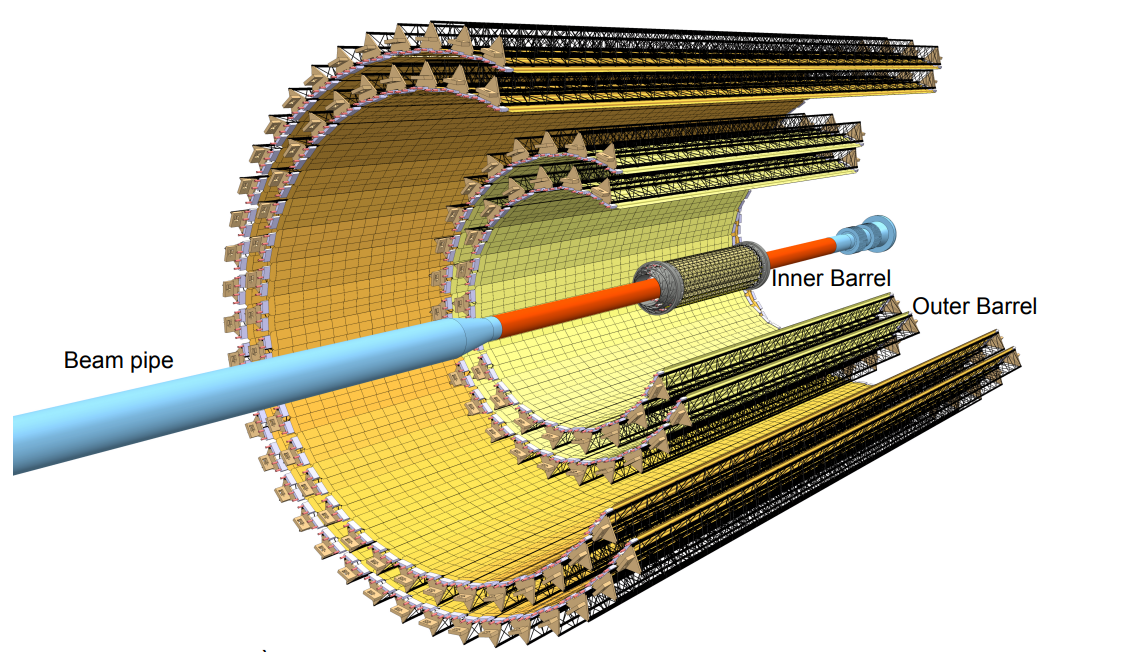
\includegraphics[width=\textwidth]{Figs/ITS_Schematic.png}
                \end{center}
            \end{figure}
        \end{column}
    \end{columns}

\end{frame}

\begin{frame}
    \frametitle{Muon Spectrometer (MCH)}

    \begin{columns}[t]
        \begin{column}{0.6\textwidth}
            \begin{itemize}
                \item Used to study various heavy particle decays via their single- and di-muon decay channels
                \item All detector material sits behind $\sim$\SI{4}{\metre} of hadronic absorber
            \end{itemize}
            \begin{figure}[h]
                \begin{center}
                    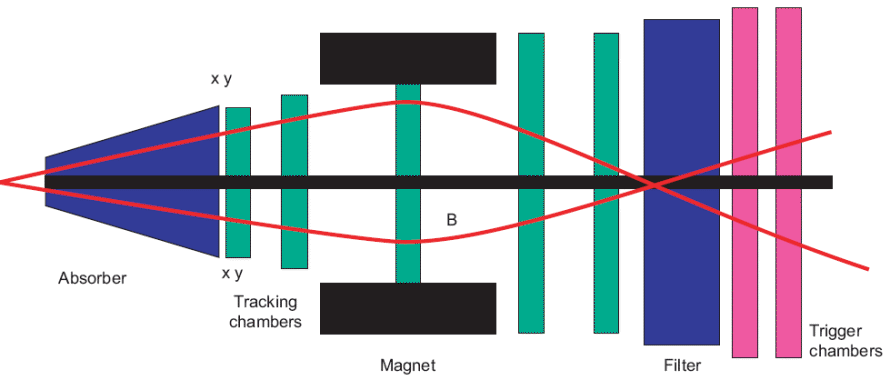
\includegraphics[width=\textwidth]{Figs/MCH_schematic.png}
                \end{center}
            \end{figure}
        \end{column}

        \begin{column}{0.4\textwidth}
            \begin{itemize}
                \item Covers $-4\leq\eta\leq -2.5$
                \item Outside the range of the ITS so previously had to perform its own tracking and vertexing
                \item Run 3 added the Muon Forward Tracker in front of the absorber to fill this role
            \end{itemize}
        \end{column}
    \end{columns}

\end{frame}

\begin{frame}
    \frametitle{Muon Forward Tracker (MFT)}

    \begin{columns}[c]
        \begin{column}{0.5\textwidth}
            \begin{itemize}
                \item Uses the same pixel detector technology as the ITS in a better-suited geometry
                \item Sits in front of the hadronic absorber, with 5 double-sided disks between \SI{-46}{\centi\metre} and \SI{-76.8}{\centi\metre}
                \item Each disk is \SI{1.4}{\centi\metre} thick
                \item Covers $-3.6\leq\eta\leq -2.45$
                \item Reconstructing a track requires hits in 4 of the 5 disks
            \end{itemize}
        \end{column}

        \begin{column}{0.5\textwidth}
            \begin{figure}[h]
                \begin{center}
                    \includegraphics[width=\textwidth]{Figs/MFT_schematic_cropped.png}
                \end{center}
            \end{figure}
        \end{column}
    \end{columns}

\end{frame}

\begin{frame}
    \frametitle{Online-Offline Analysis Framework (O2)}

    \begin{columns}[c]
        \begin{column}{0.6\textwidth}
            \begin{itemize}
                \item Created for Run 3 to deal with untriggered data capture, splitting it into \SI{10}{\milli\second} ``timeframes'' in online processing, then compressed timeframes (CTFs), which are saved to disk
                \item Raw data converted to usable data with ``reconstruction passes'' in the offline stage, producing Analysis Object Data (AOD) files
                \item Then analysed with C\texttt{++} and ROOT to make the most of computational resources and to minimise disk space usage
                \item Don't breathe near O2, or it might break
            \end{itemize}
        \end{column}

        \begin{column}{0.4\textwidth}
            \begin{figure}
                \begin{center}
                    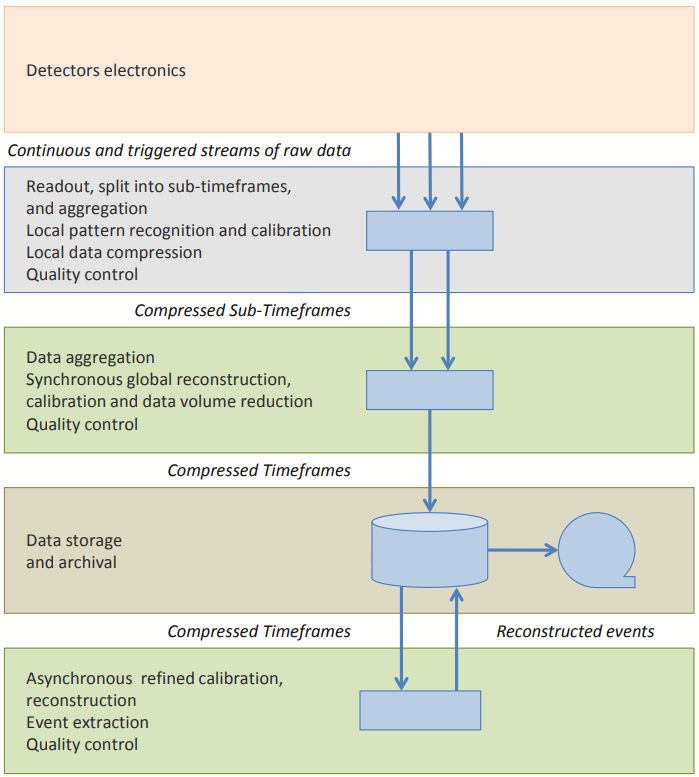
\includegraphics[width=\textwidth]{Figs/O2_flow.png}
                \end{center}
            \end{figure}
        \end{column}
    \end{columns}

\end{frame}

\section{Data \& Results}

\begin{frame}
    \frametitle{What data are we using?}

    \begin{itemize}
        \item Pilot beam runs 505548 and 505645 from October 2021
        \item Non-nominal centre of mass energy $\sqrt{s}=\SI{900}{\giga\electronvolt}$
        \item Detectors running: ITS, MCH, MFT, MID, TOF, TPC, TRD
        \item All plots include data from both runs
        \item We used data from two different reconstruction passes
    \end{itemize}

\end{frame}

\begin{frame}
    \frametitle{MFT Kinematics (pass 3)}

    \begin{columns}
        \begin{column}{0.5\textwidth}
            \vspace*{-0.43cm}
            \begin{figure}
                \begin{center}
                    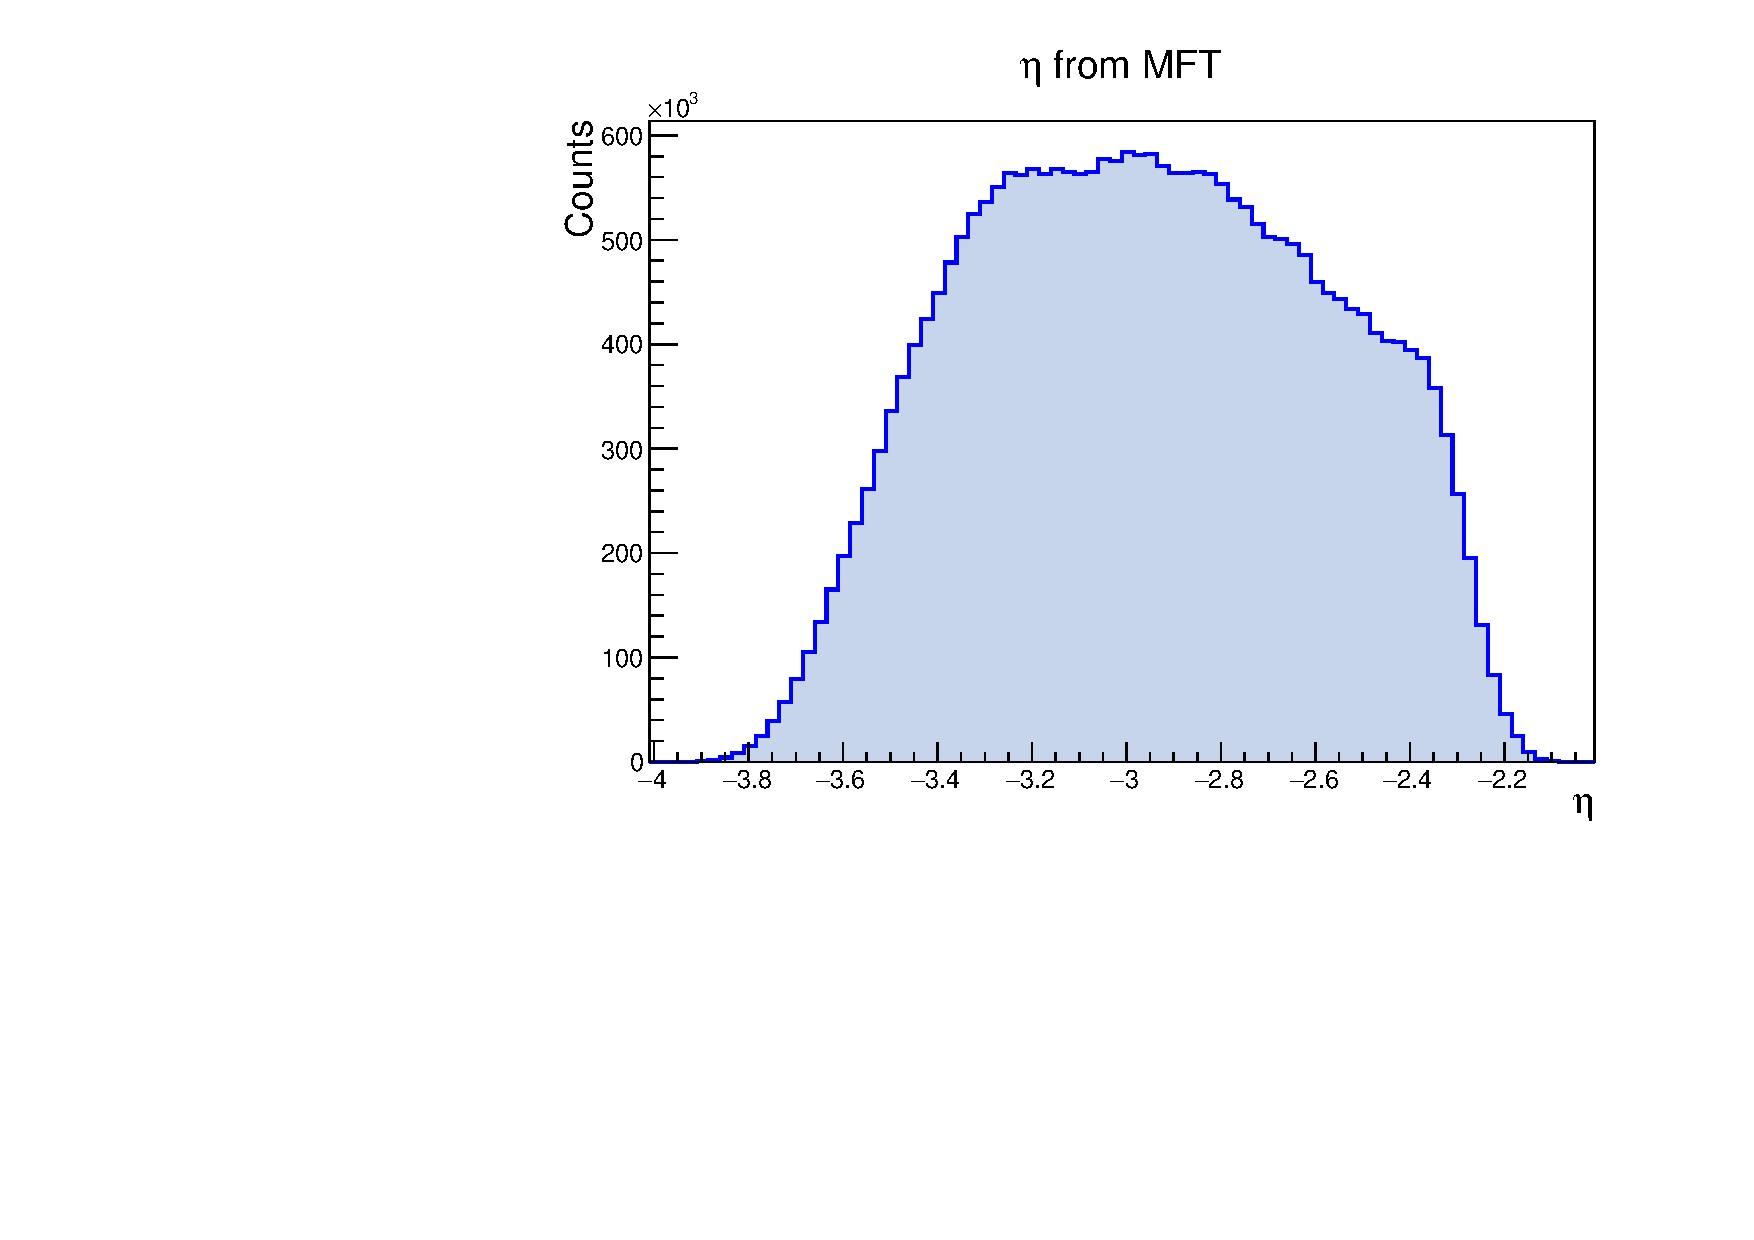
\includegraphics[width=0.95\textwidth]{Plots/pass3_MFT/MFTeta_pass3.pdf}
                \end{center}
            \end{figure}
            \vspace*{-0.6cm}
            \begin{figure}
                \begin{center}
                    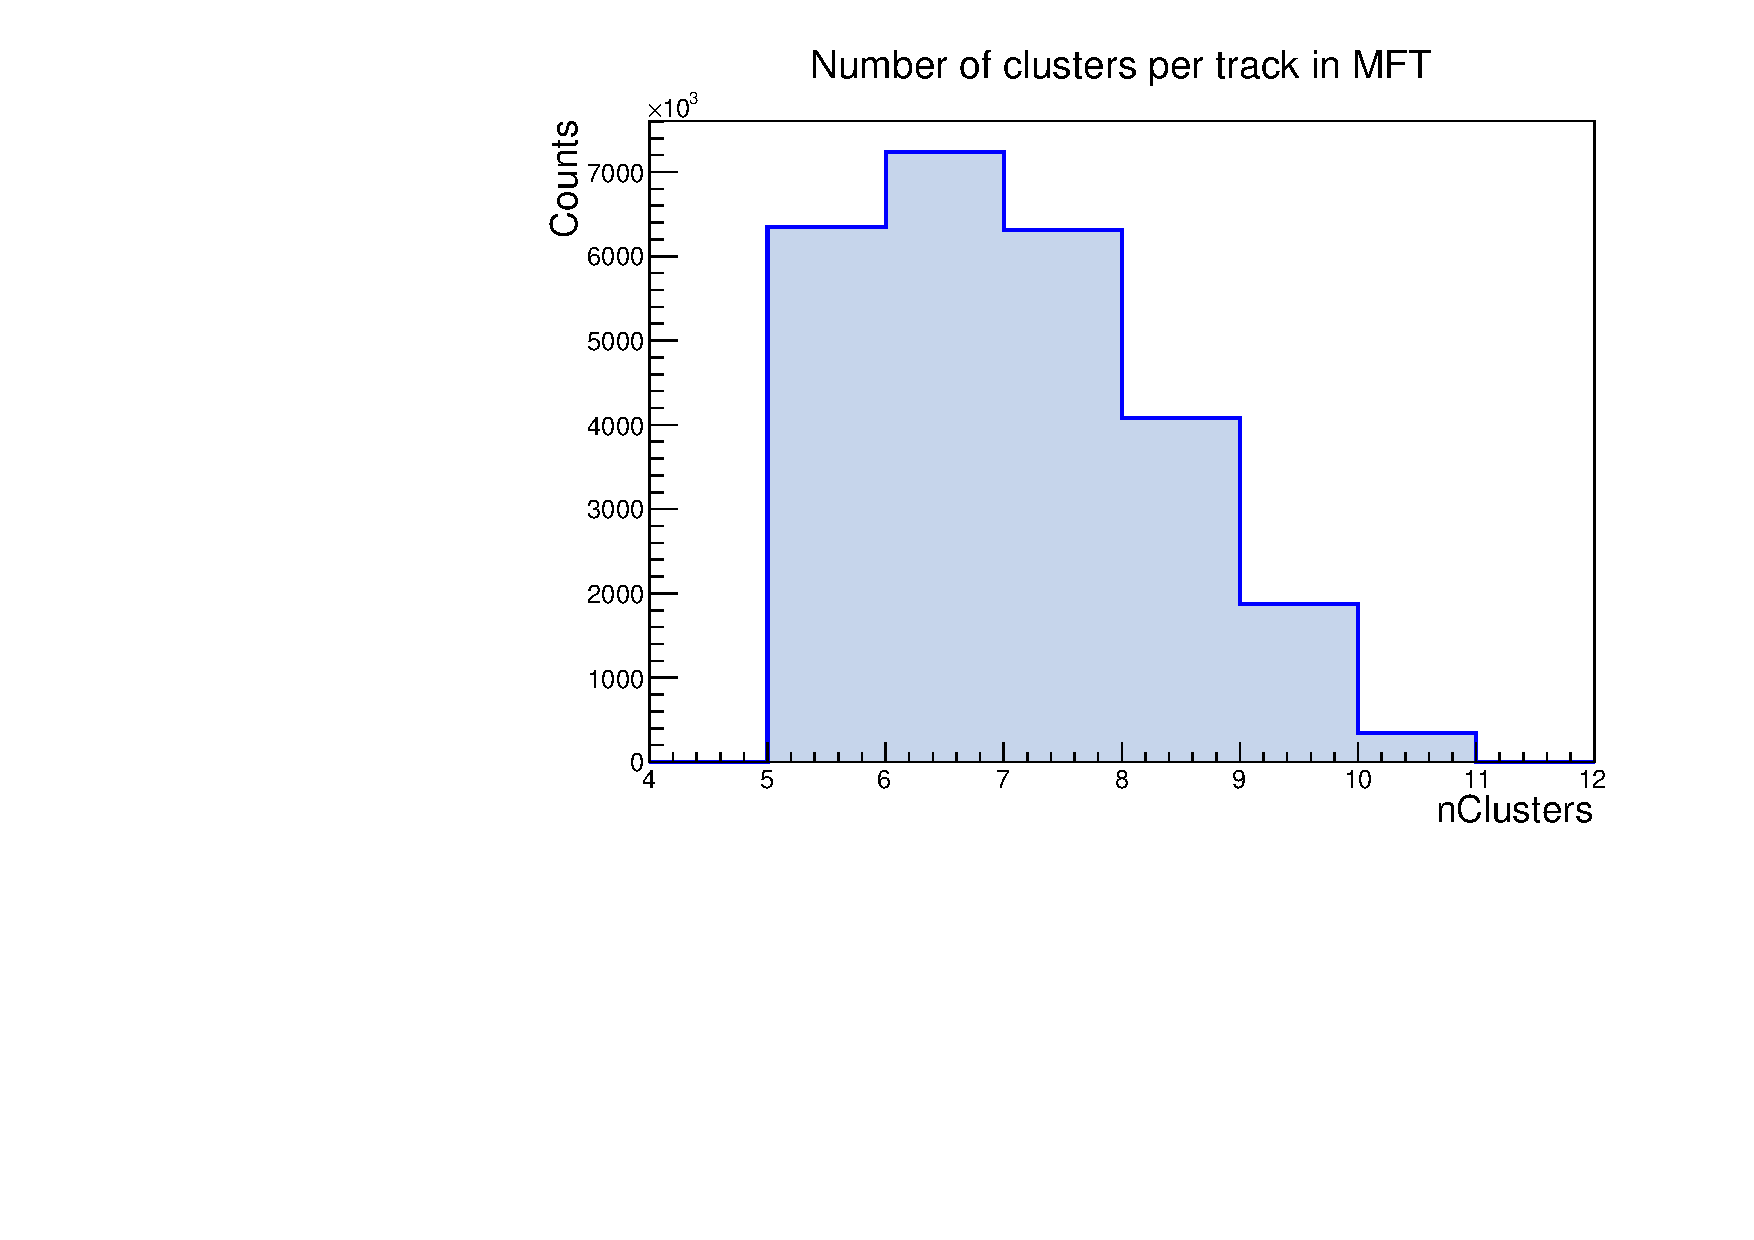
\includegraphics[width=0.95\textwidth]{Plots/pass3_MFT/nClusters_pass3.pdf}
                \end{center}
            \end{figure}
        \end{column}
        \begin{column}{0.5\textwidth}
            \vspace*{-0.43cm}
            \begin{figure}
                \begin{center}
                    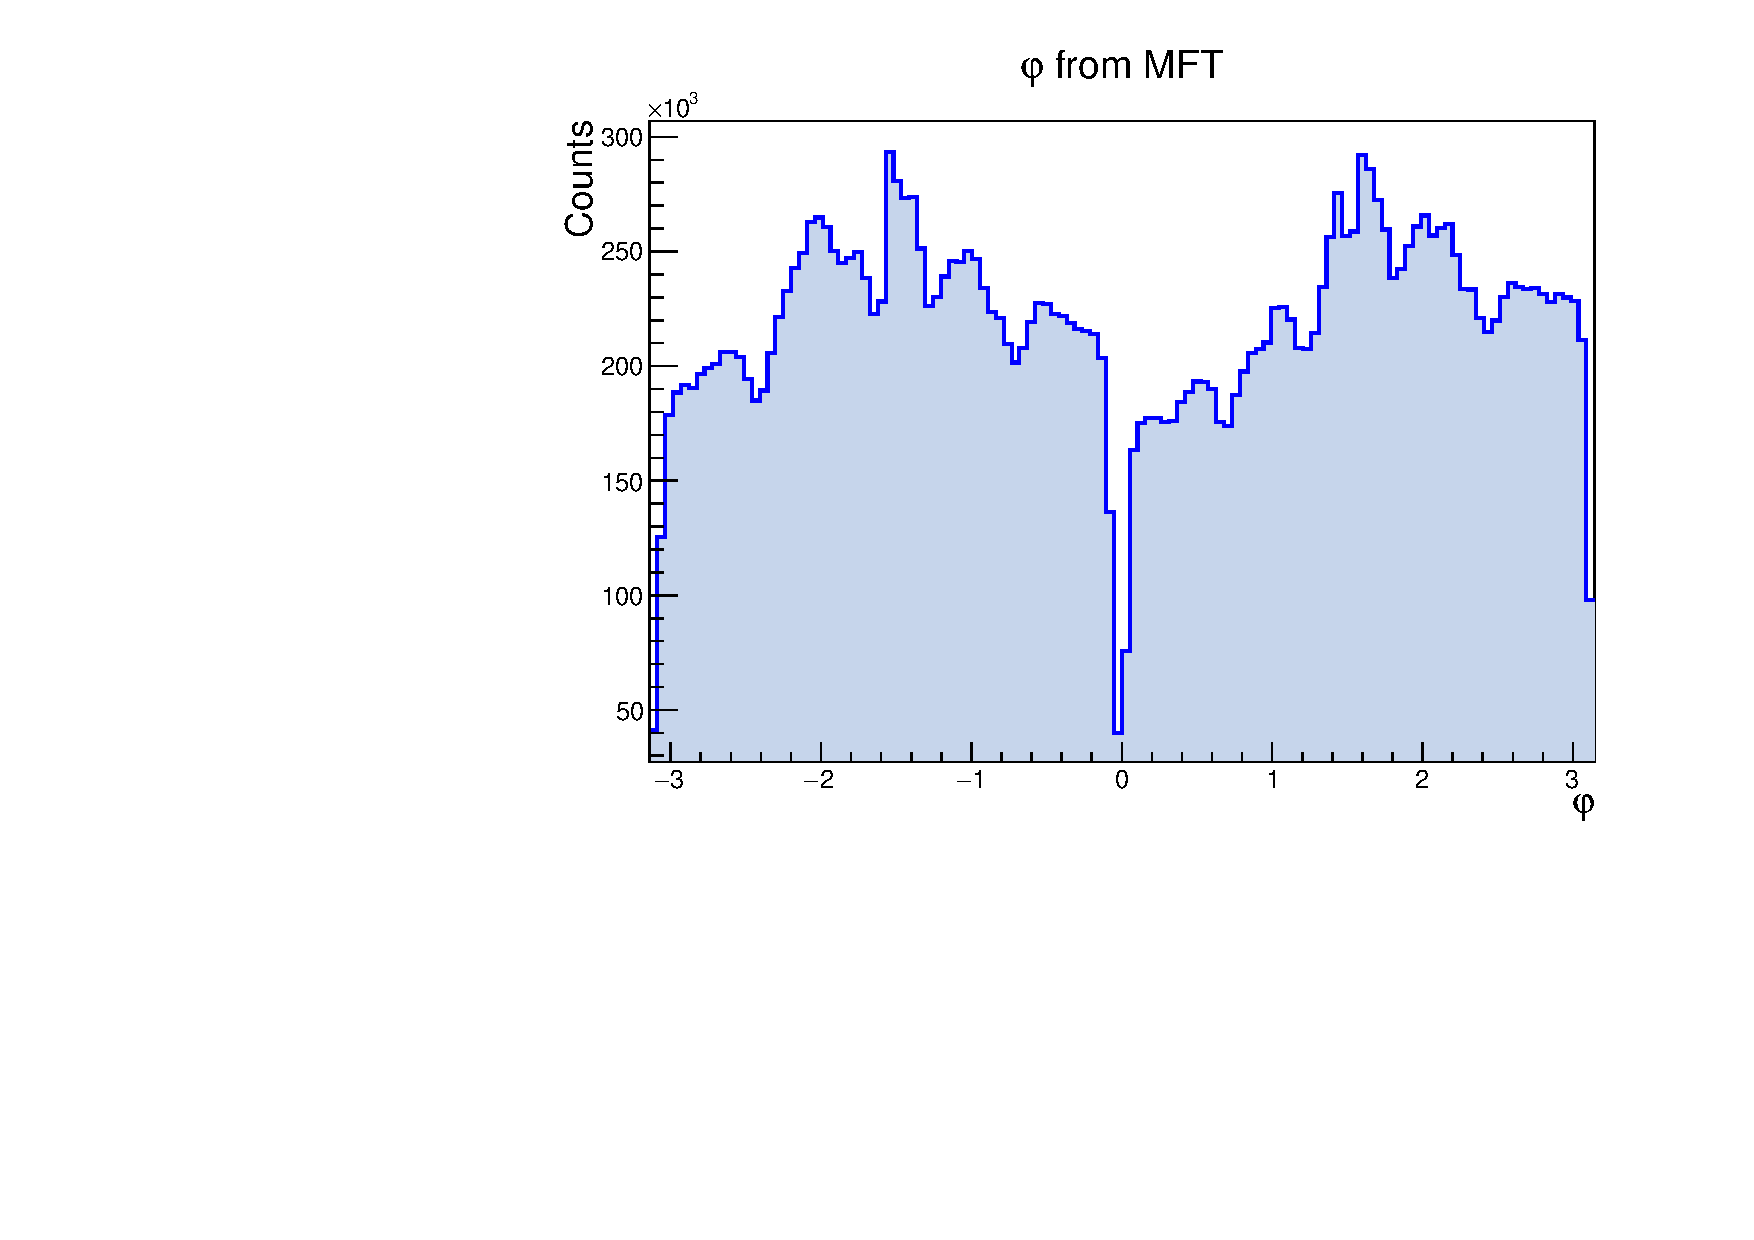
\includegraphics[width=0.95\textwidth]{Plots/pass3_MFT/phi_pass3.pdf}
                \end{center}
            \end{figure}
            \vspace*{-0.6cm}
            \begin{figure}
                \begin{center}
                    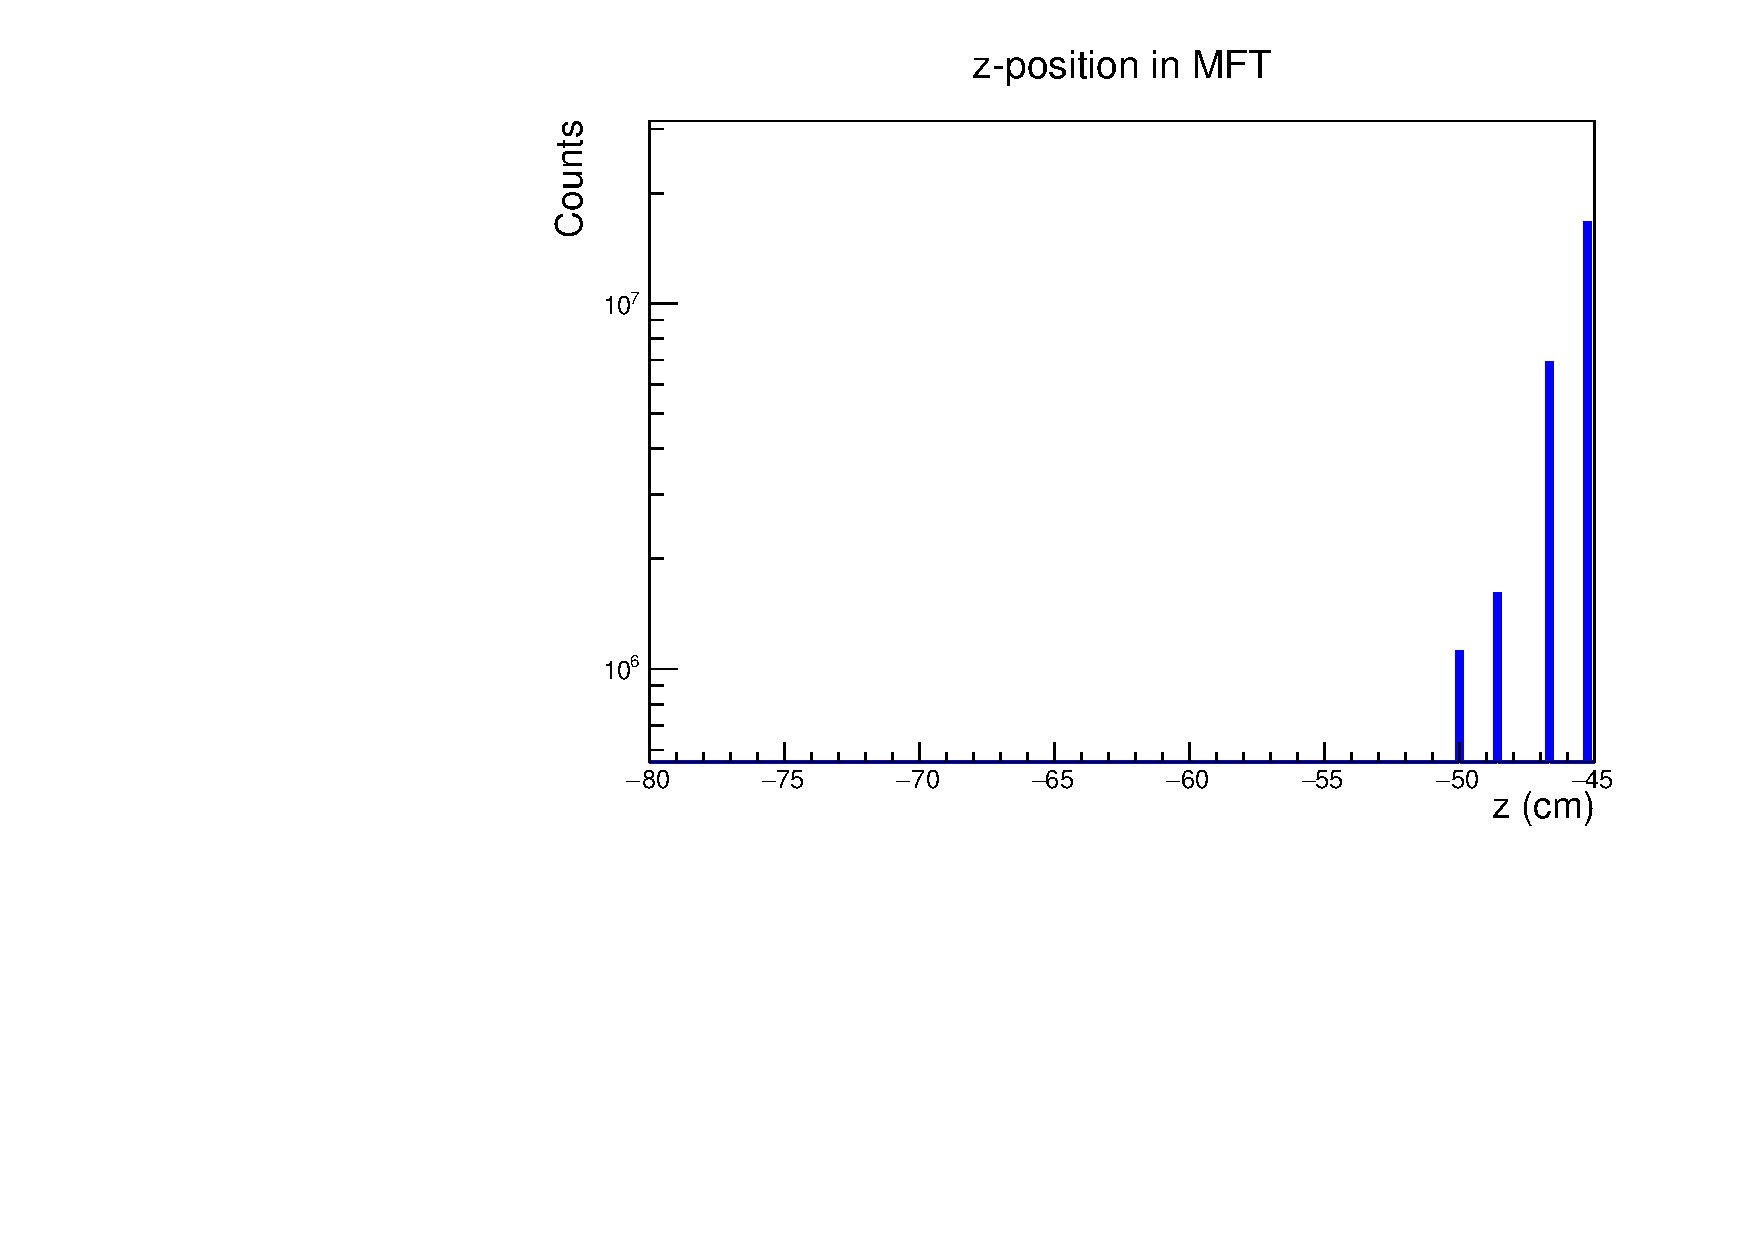
\includegraphics[width=0.95\textwidth]{Plots/pass3_MFT/Z_MFT_pass3.pdf}
                \end{center}
            \end{figure}
        \end{column}
    \end{columns}

\end{frame}

\begin{frame}
    \frametitle{MFT x-y Plots (pass 3)}

    \begin{columns}[T]
        \begin{column}{0.5\textwidth}
            \vspace*{-0.5cm}
            \begin{figure}
                \begin{center}
                    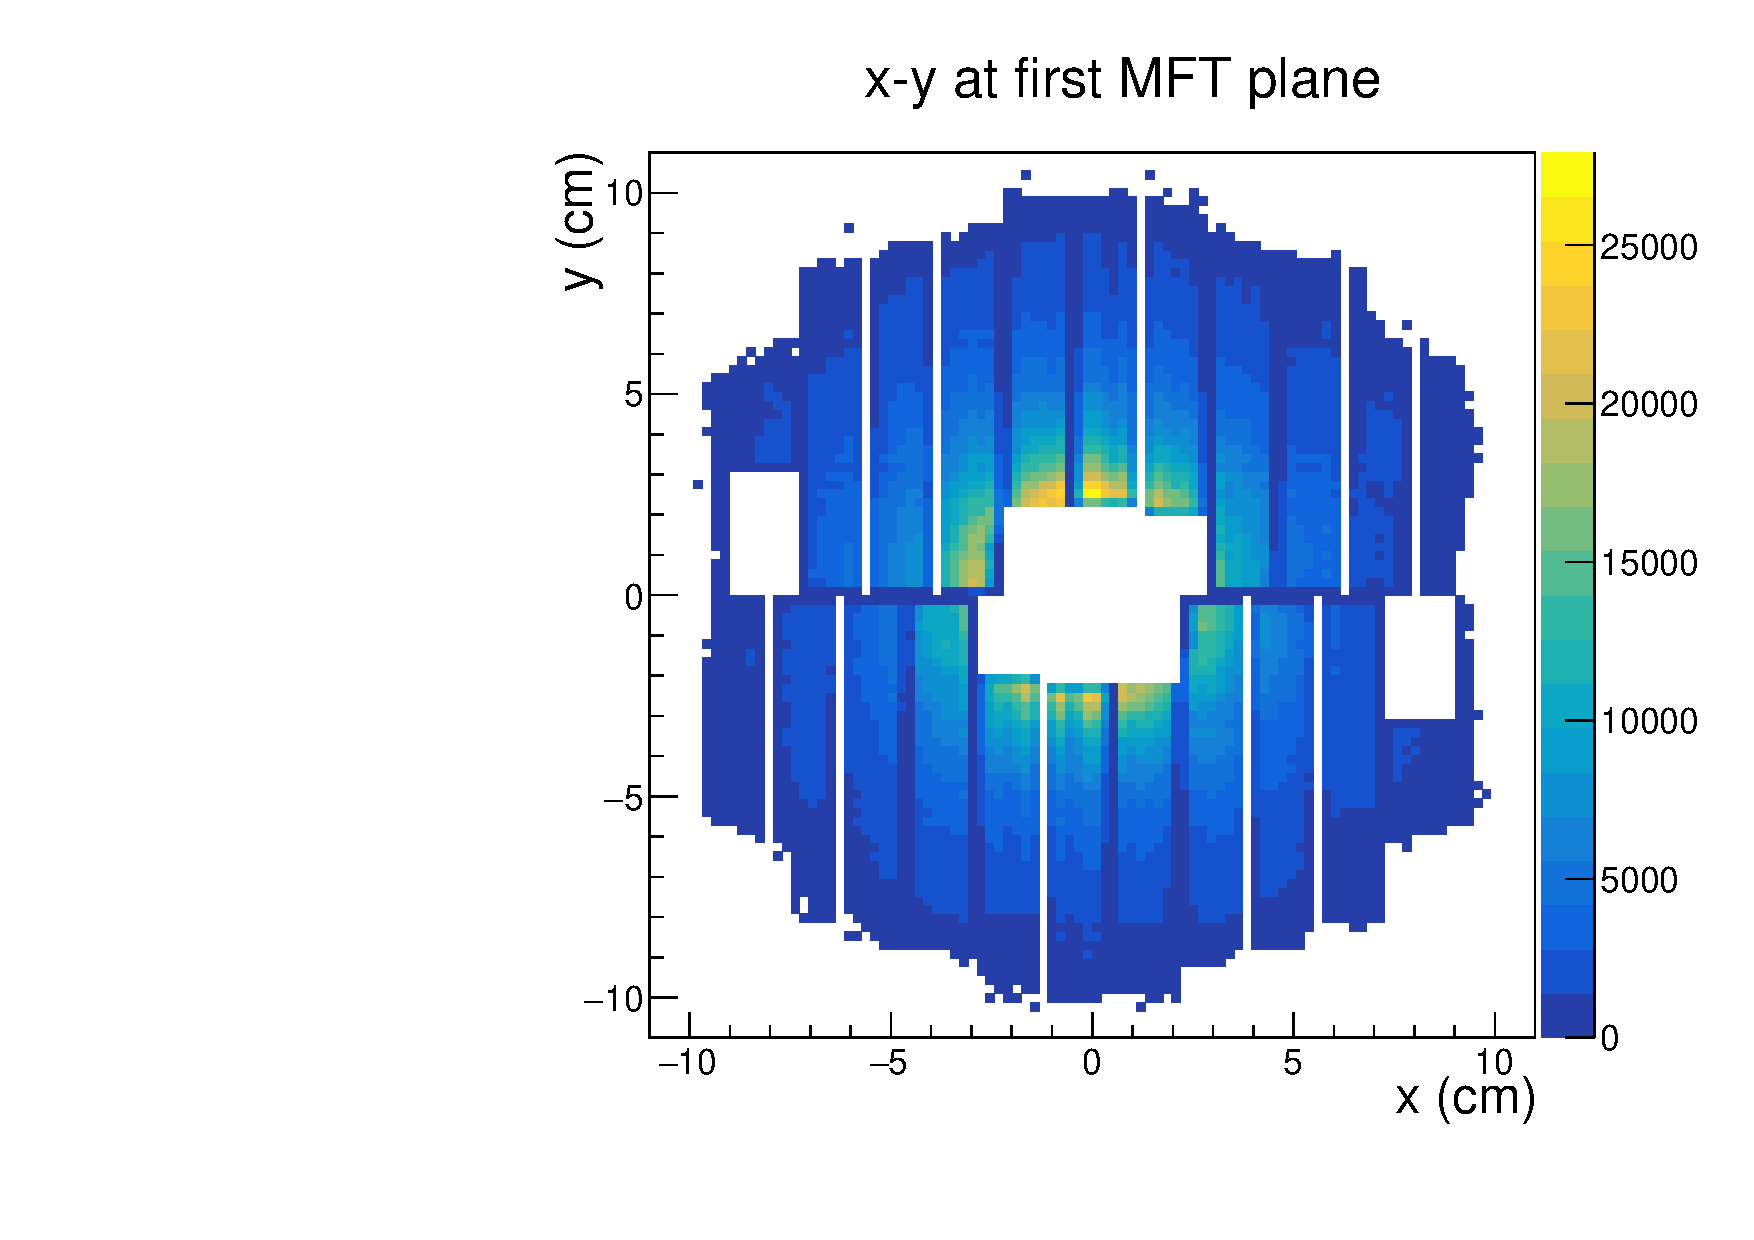
\includegraphics[width=0.7\textwidth]{Plots/pass3_MFT/x_y_1_pass3.pdf}
                \end{center}
            \end{figure}
            \vspace*{-0.7cm}
            \begin{figure}
                \begin{center}
                    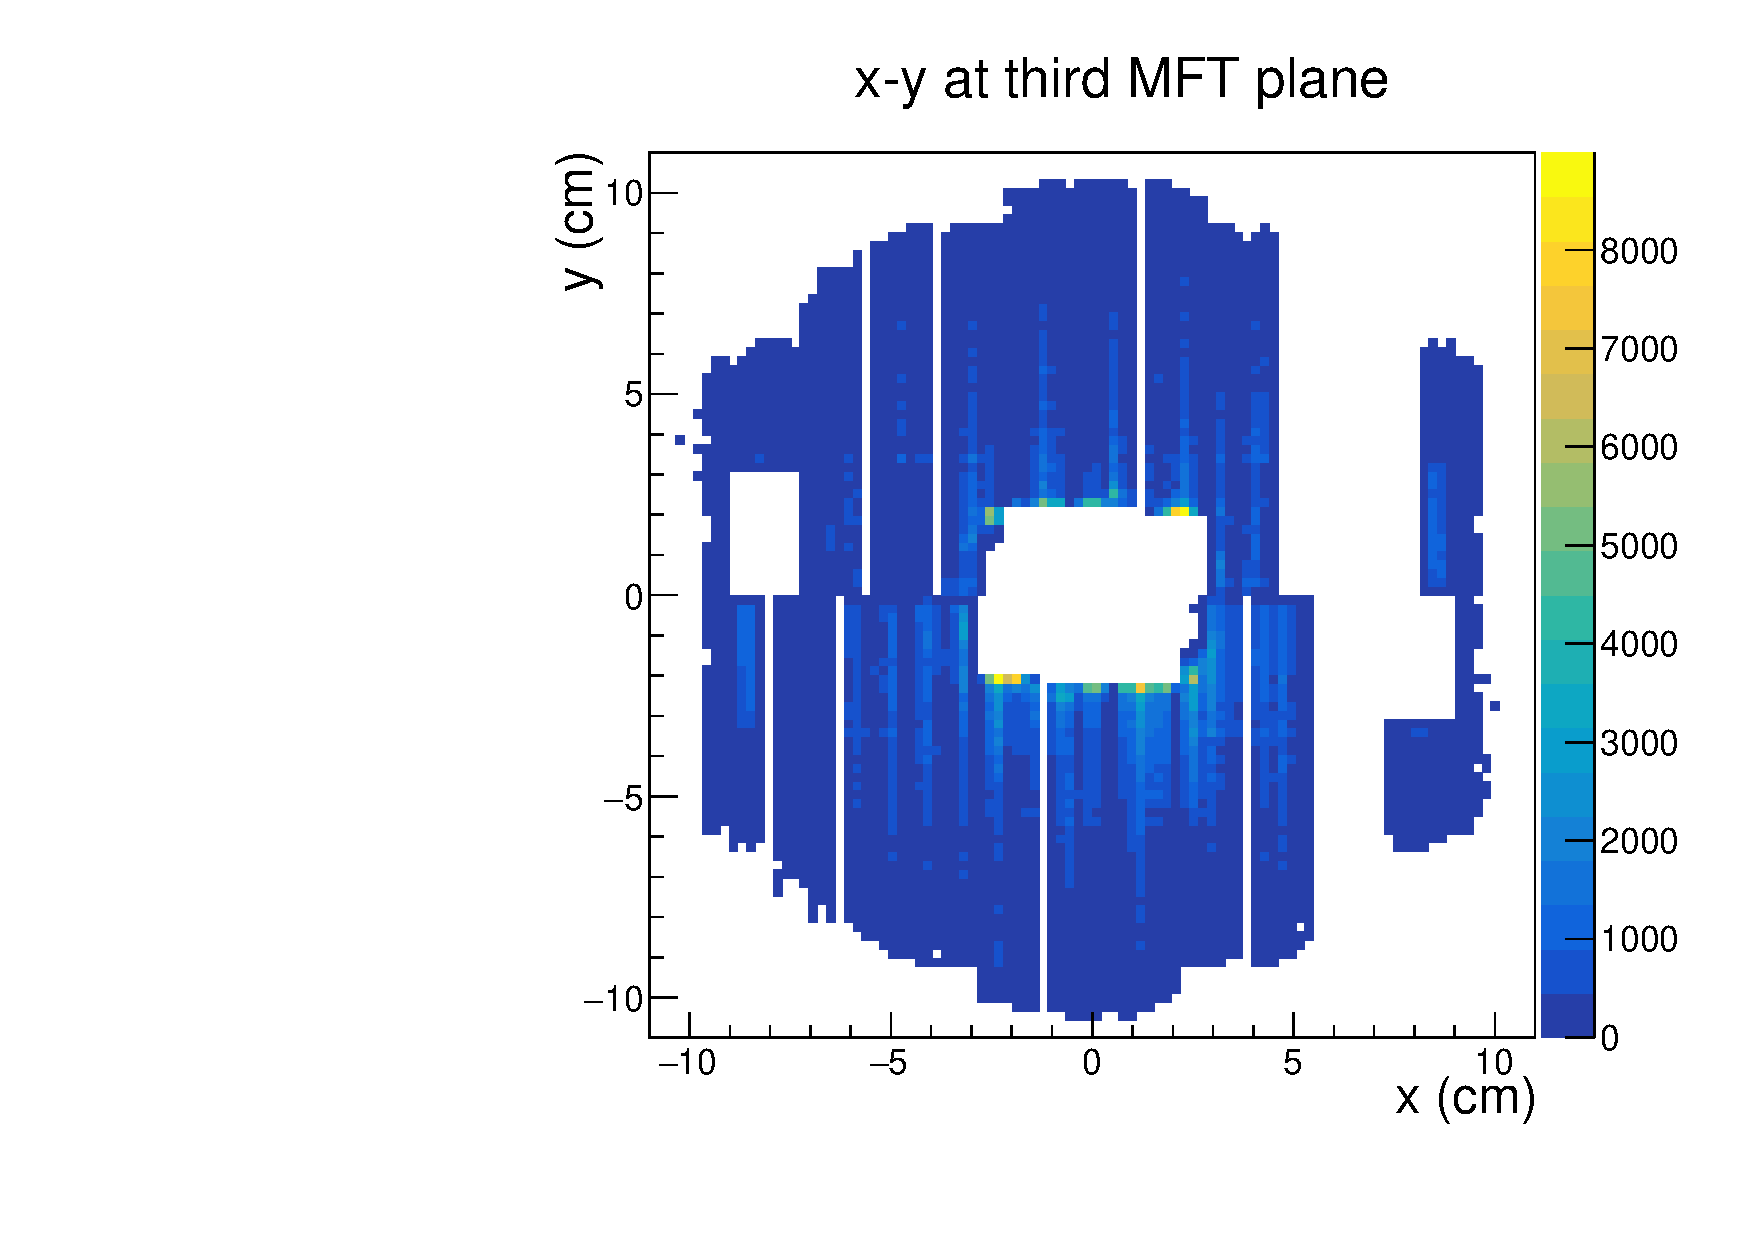
\includegraphics[width=0.7\textwidth]{Plots/pass3_MFT/x_y_3_pass3.pdf}
                \end{center}
            \end{figure}
        \end{column}
        \begin{column}{0.5\textwidth}
            \vspace*{-0.5cm}
            \begin{figure}
                \begin{center}
                    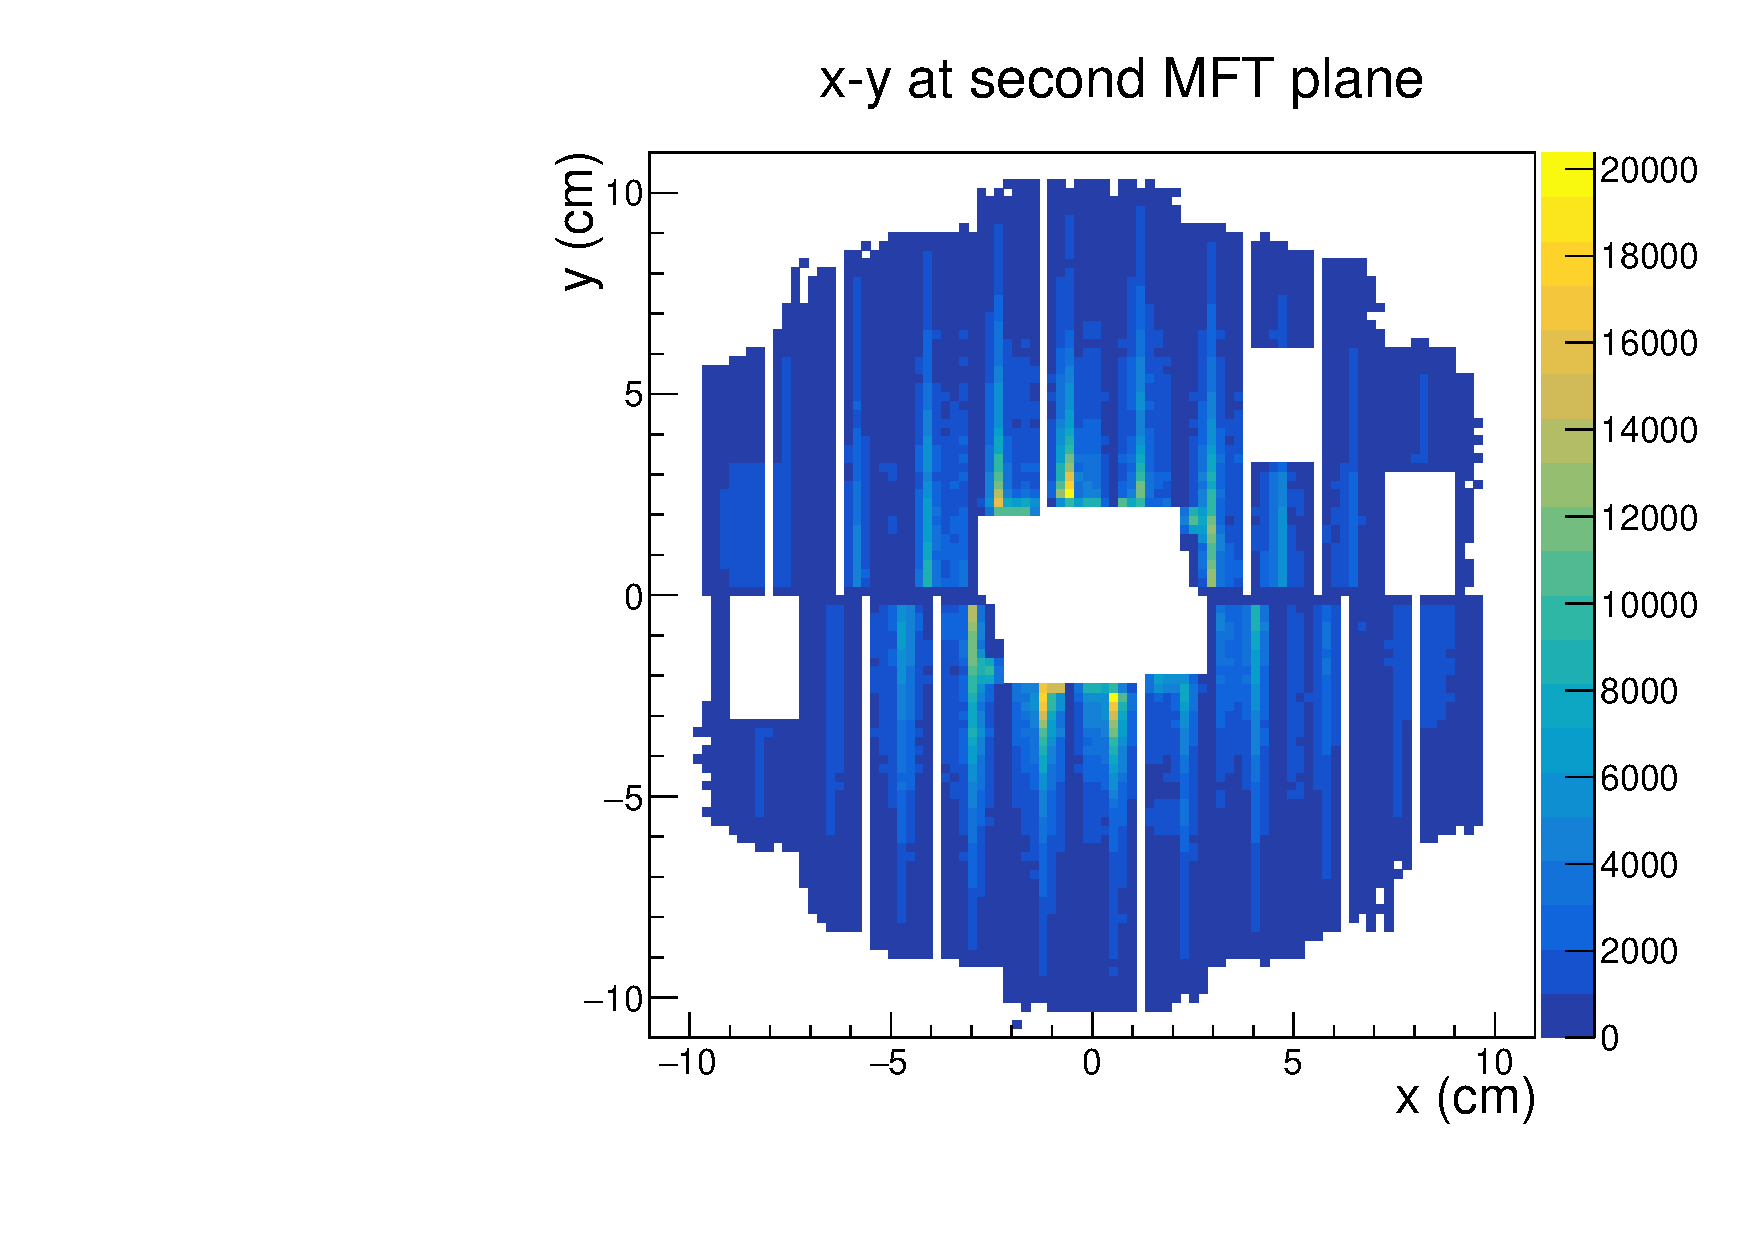
\includegraphics[width=0.7\textwidth]{Plots/pass3_MFT/x_y_2_pass3.pdf}
                \end{center}
            \end{figure}
            \vspace*{-0.7cm}
            \begin{figure}
                \begin{center}
                    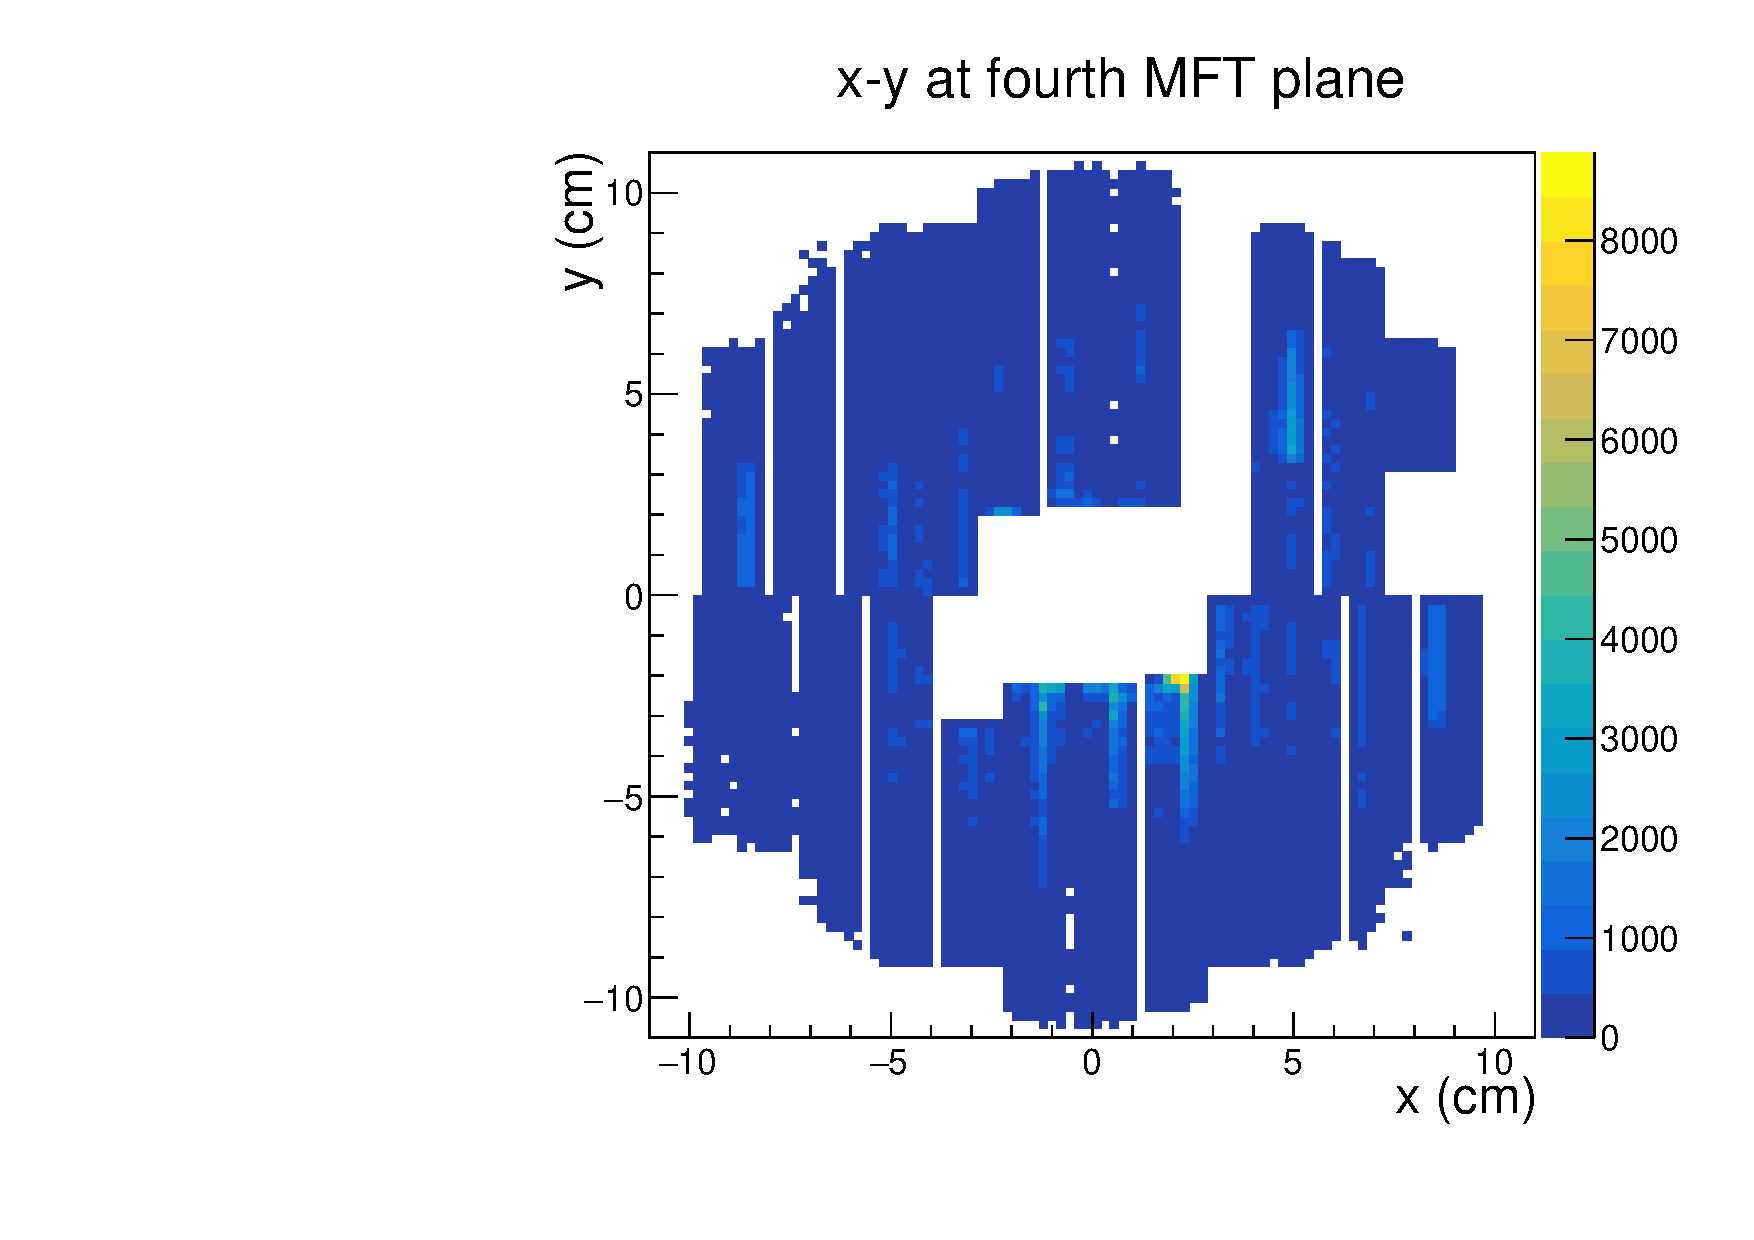
\includegraphics[width=0.7\textwidth]{Plots/pass3_MFT/x_y_4_pass3.pdf}
                \end{center}
            \end{figure}
        \end{column}
    \end{columns}

\end{frame}

\begin{frame}
    \frametitle{$\eta$-$\varphi$ in the MFT (pass 3)}
        \begin{figure}
            \begin{center}
                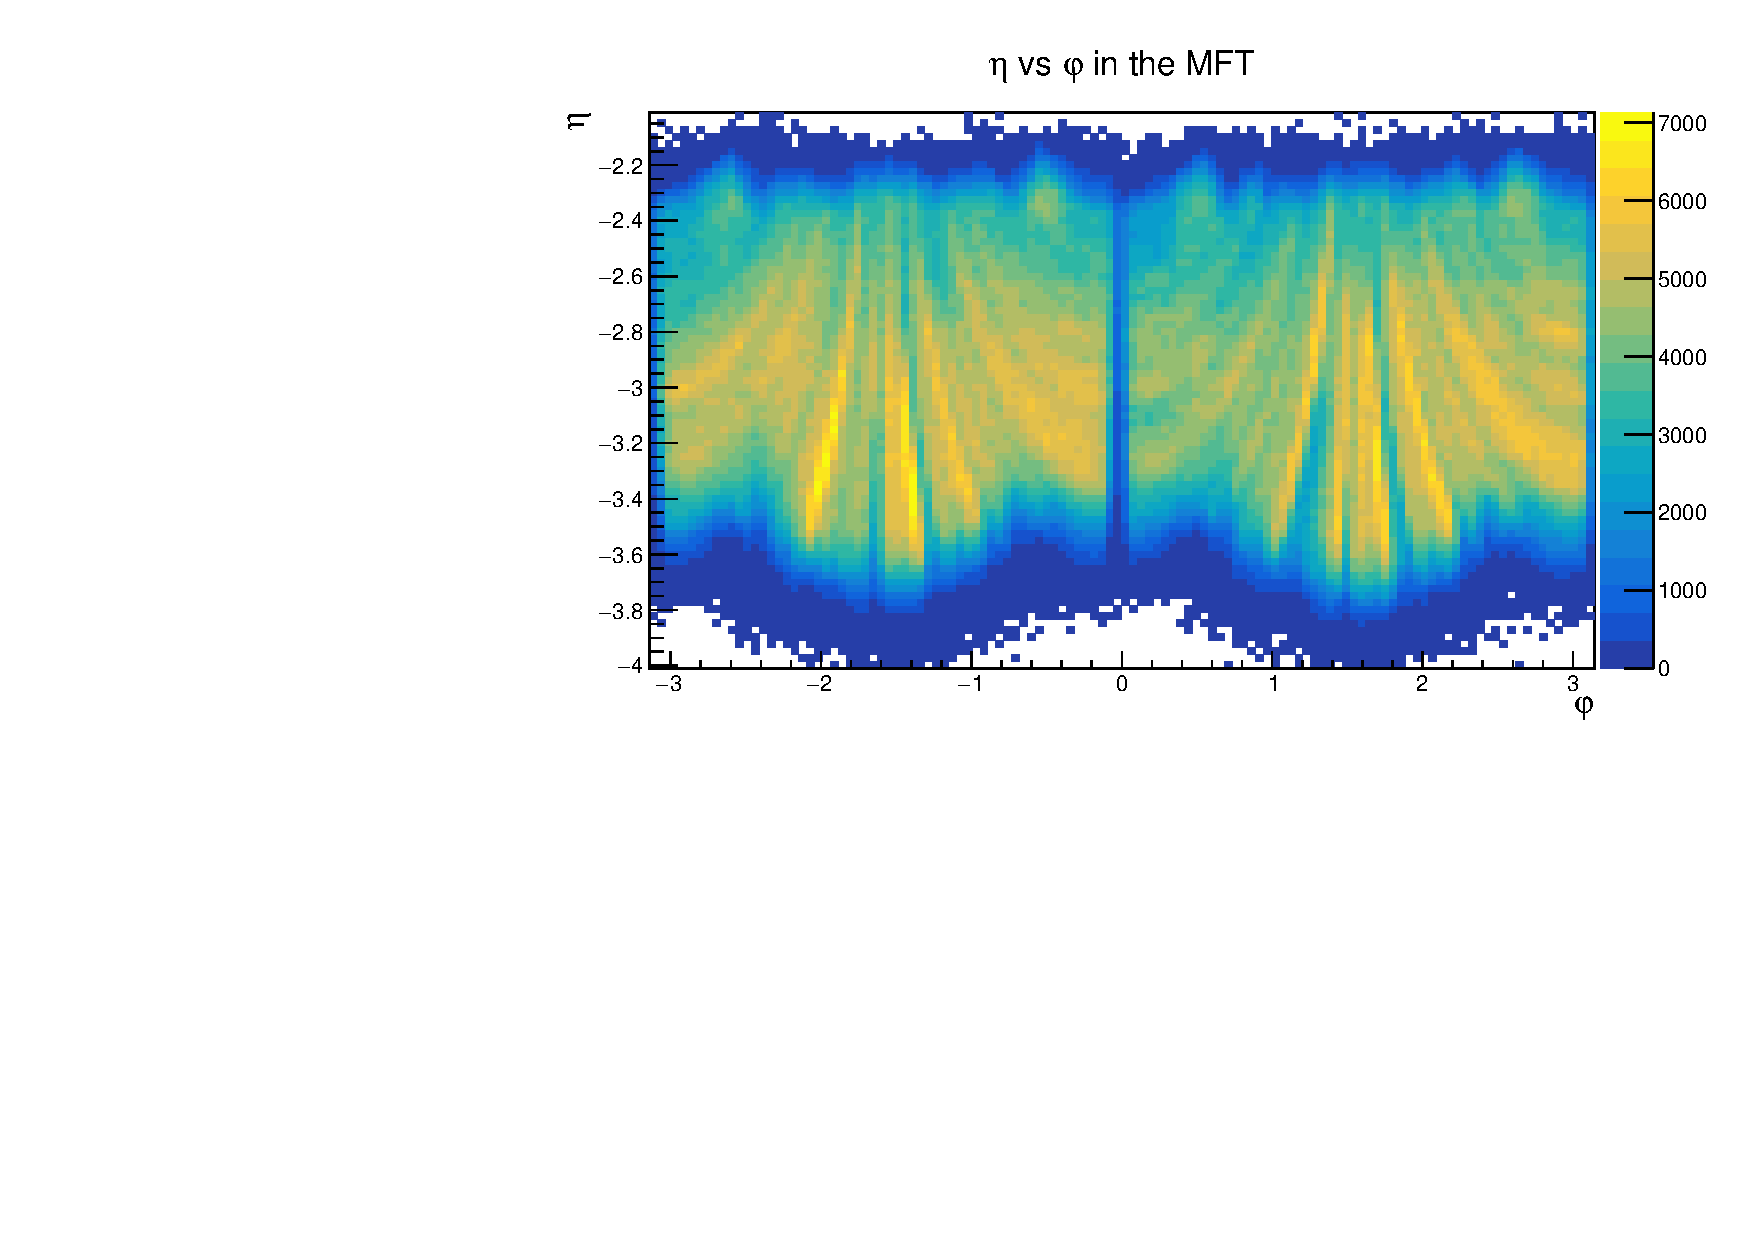
\includegraphics[width=\textwidth]{Plots/pass3_MFT/eta_phi_pass3.pdf}
            \end{center}
        \end{figure}
\end{frame}

\begin{frame}
    \frametitle{Comparison of $\eta$ for pass 3 and pass 4 in the MFT}
        \begin{figure}
            \begin{center}
                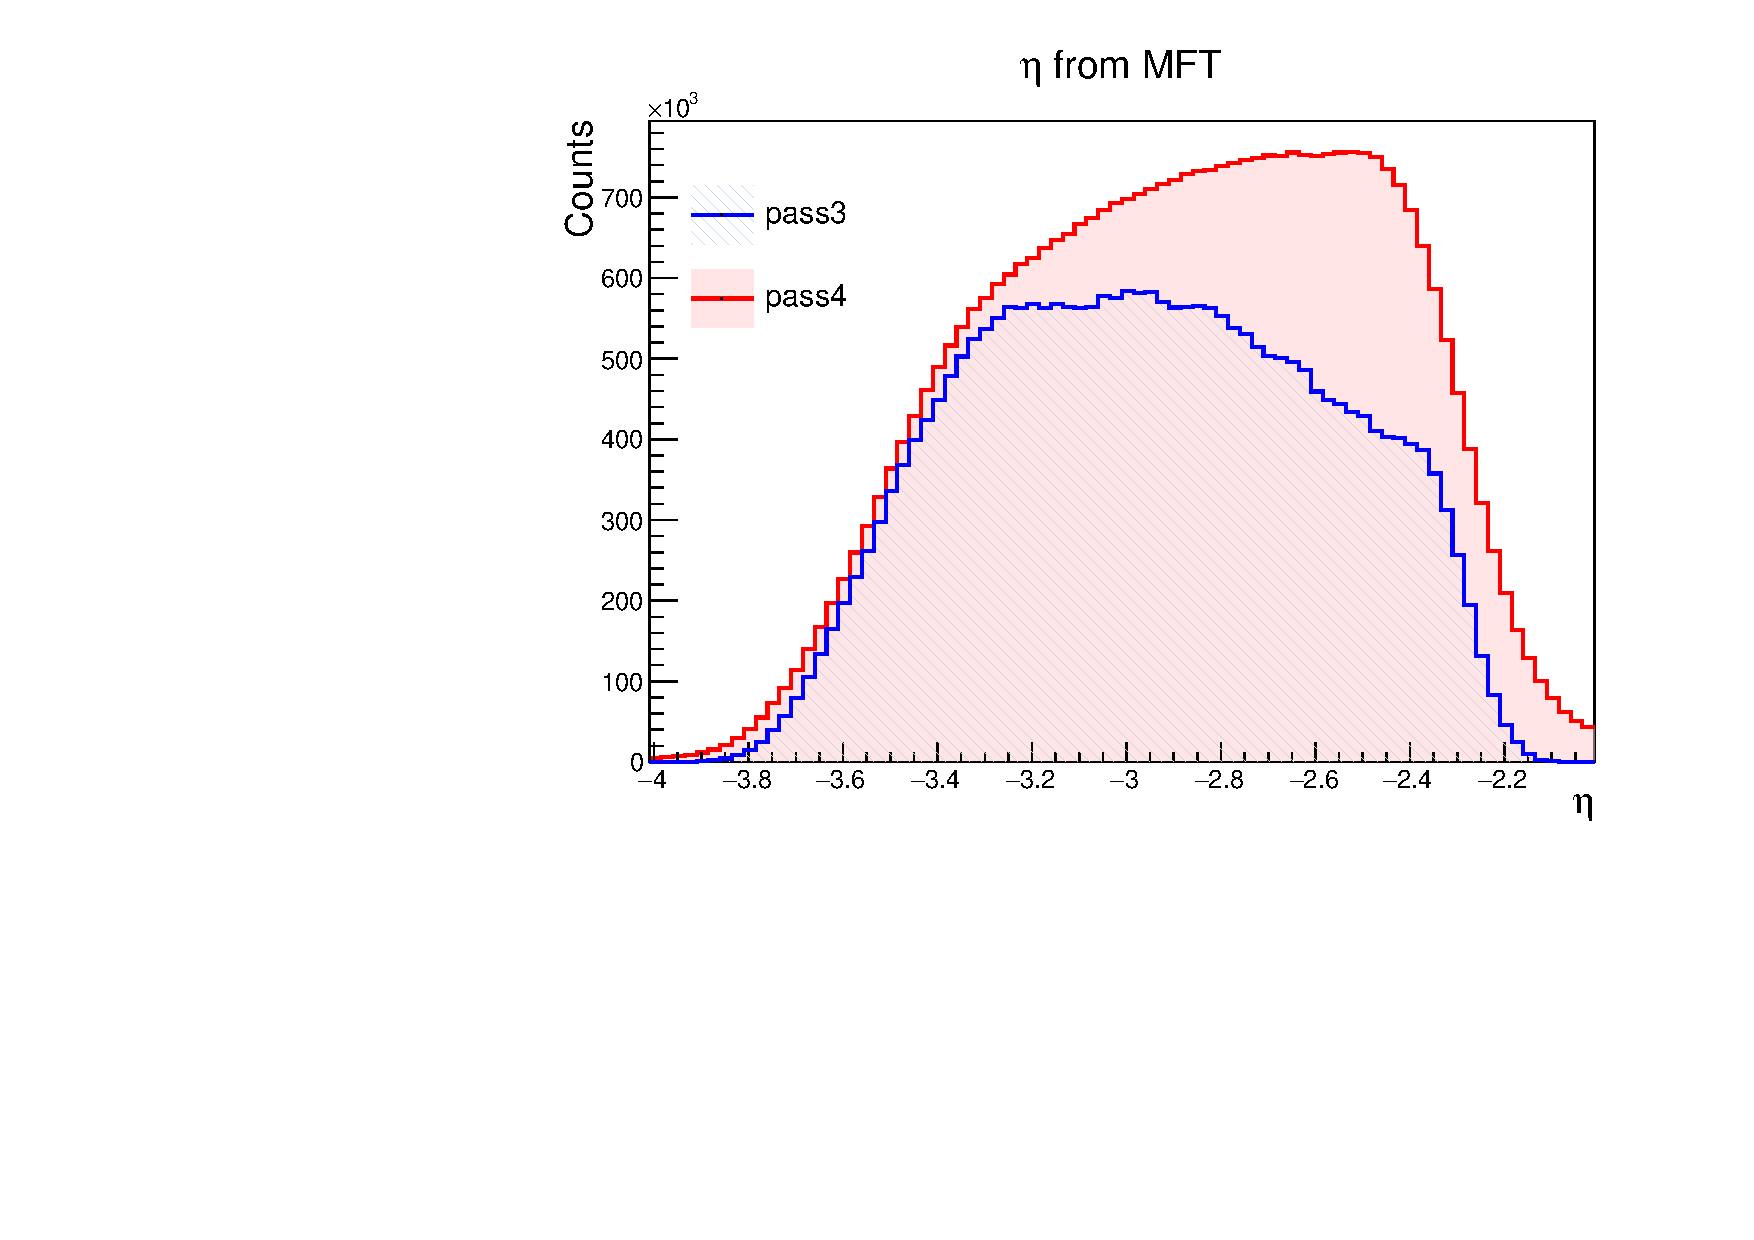
\includegraphics[width=0.9\textwidth]{Plots/pass3_pass4.pdf}
            \end{center}
        \end{figure}
\end{frame}

\begin{frame}
    \frametitle{ITS Kinematics (pass 4, hasITS)}

    \begin{columns}
        \begin{column}{0.5\textwidth}
            \vspace*{-0.43cm}
            \begin{figure}
                \begin{center}
                    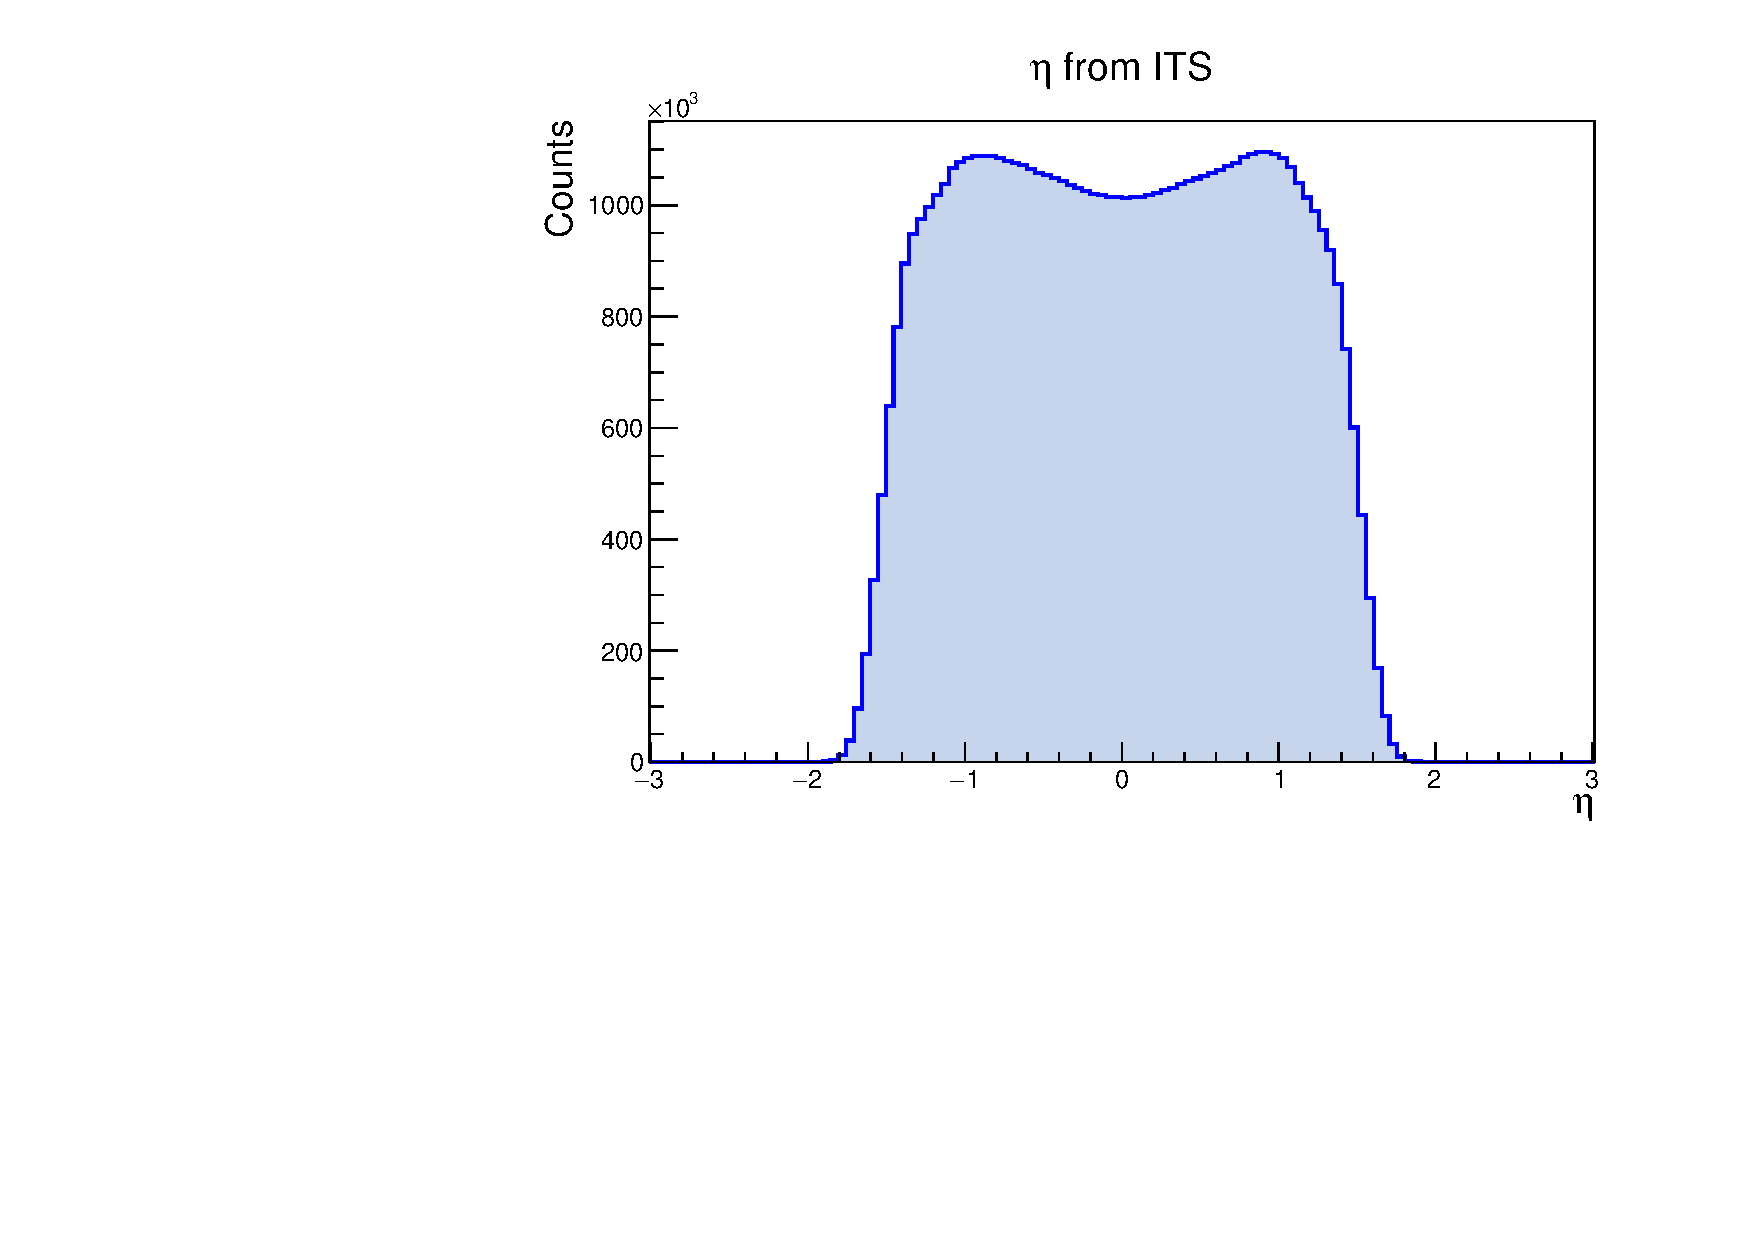
\includegraphics[width=0.95\textwidth]{Plots/pass4_TracksIU/eta.pdf}
                \end{center}
            \end{figure}
            \vspace*{-0.6cm}
            \begin{figure}
                \begin{center}
                    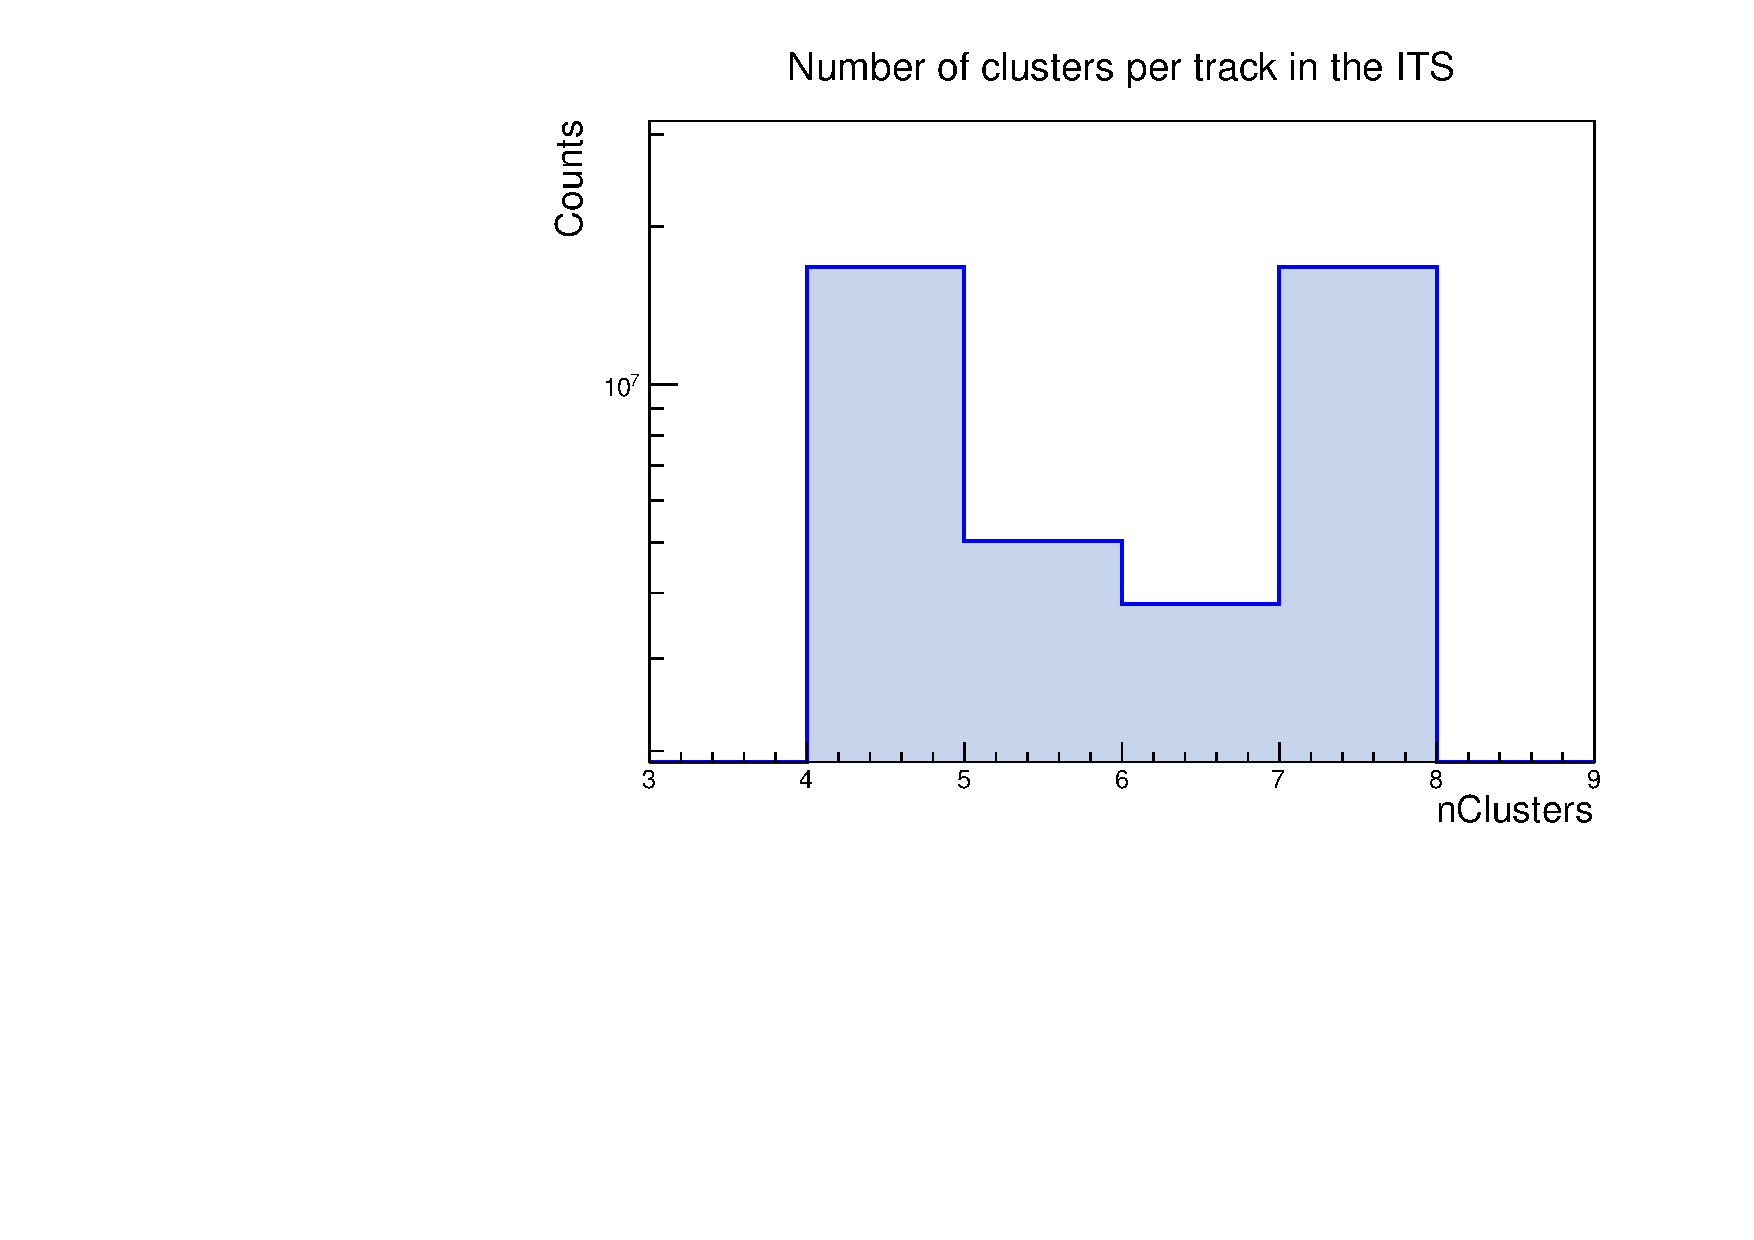
\includegraphics[width=0.95\textwidth]{Plots/pass4_TracksIU/itsNCls.pdf}
                \end{center}
            \end{figure}
        \end{column}
        \begin{column}{0.5\textwidth}
            \vspace*{-0.43cm}
            \begin{figure}
                \begin{center}
                    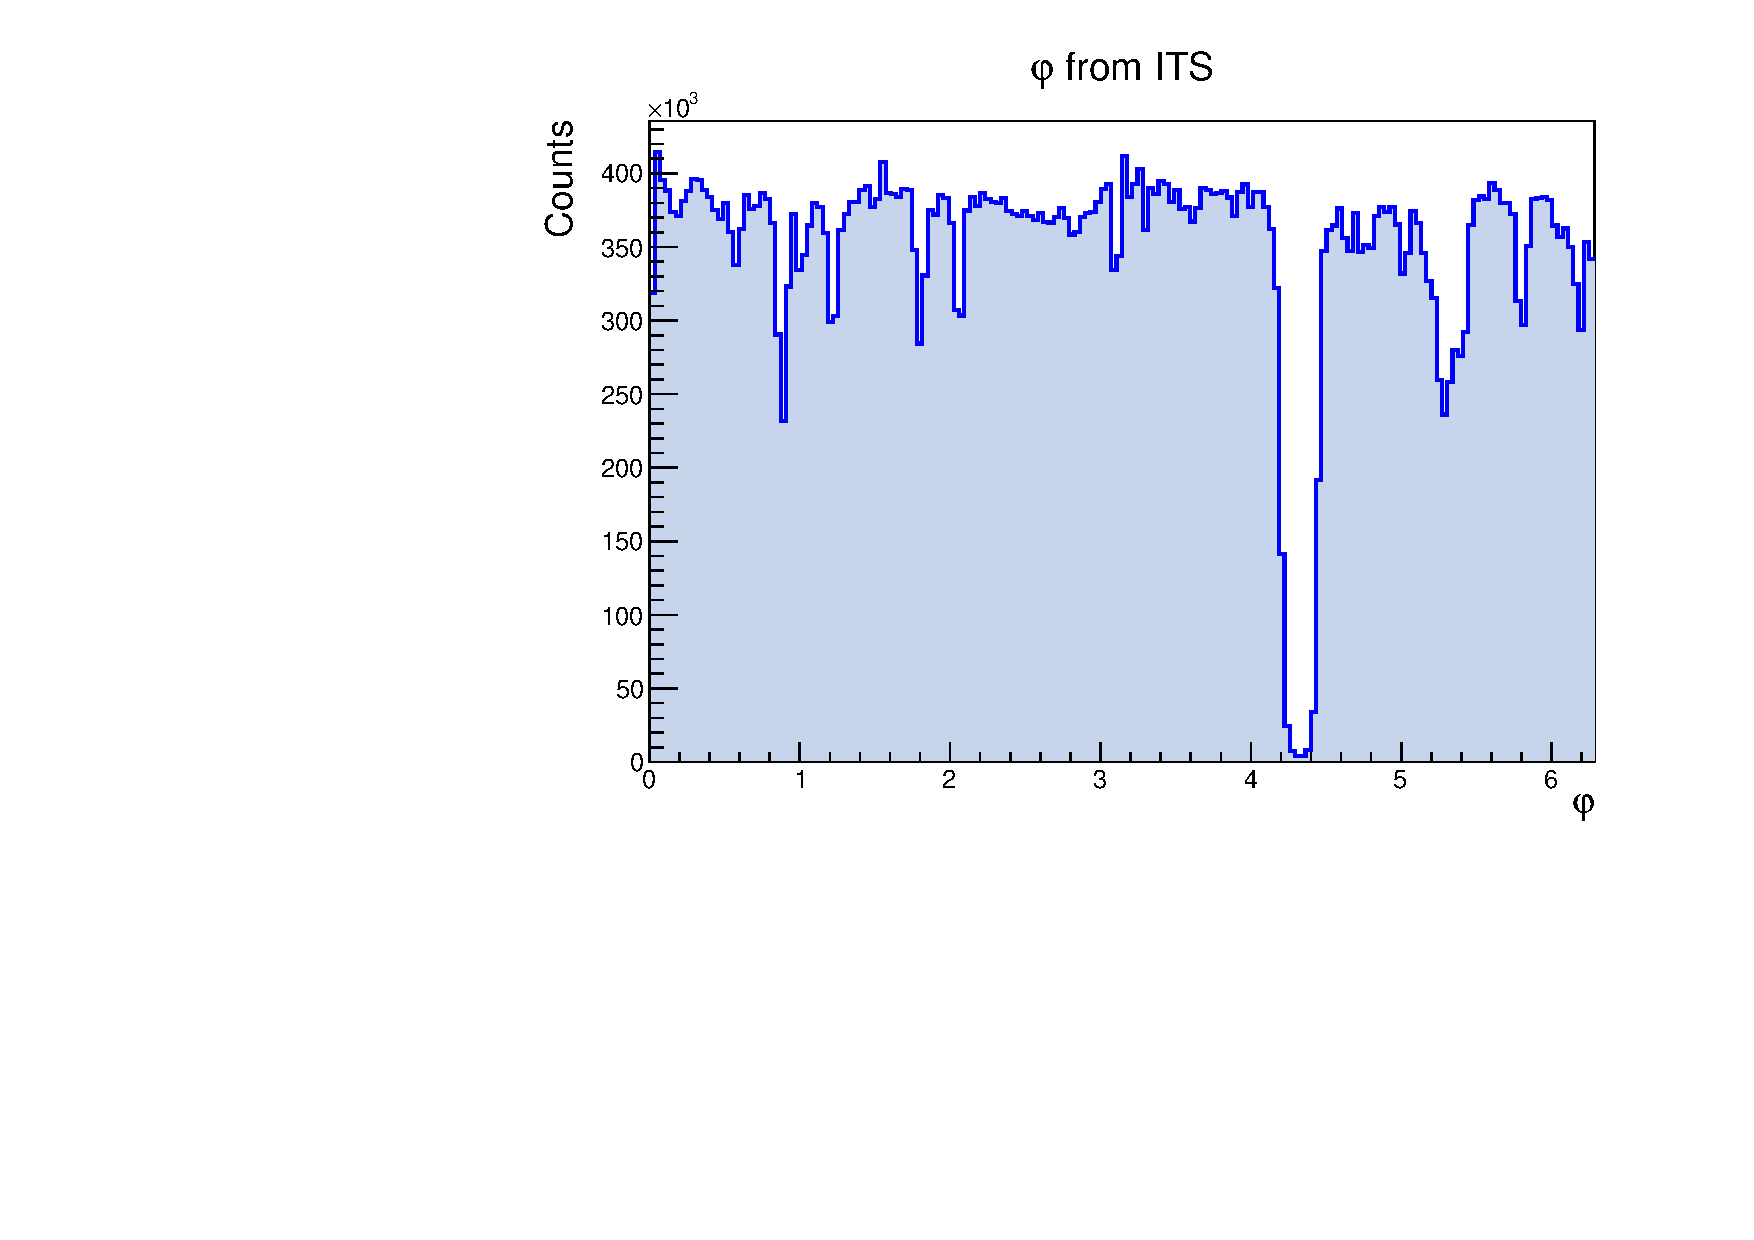
\includegraphics[width=0.95\textwidth]{Plots/pass4_TracksIU/phi.pdf}
                \end{center}
            \end{figure}
            \vspace*{-0.6cm}
            \begin{figure}
                \begin{center}
                    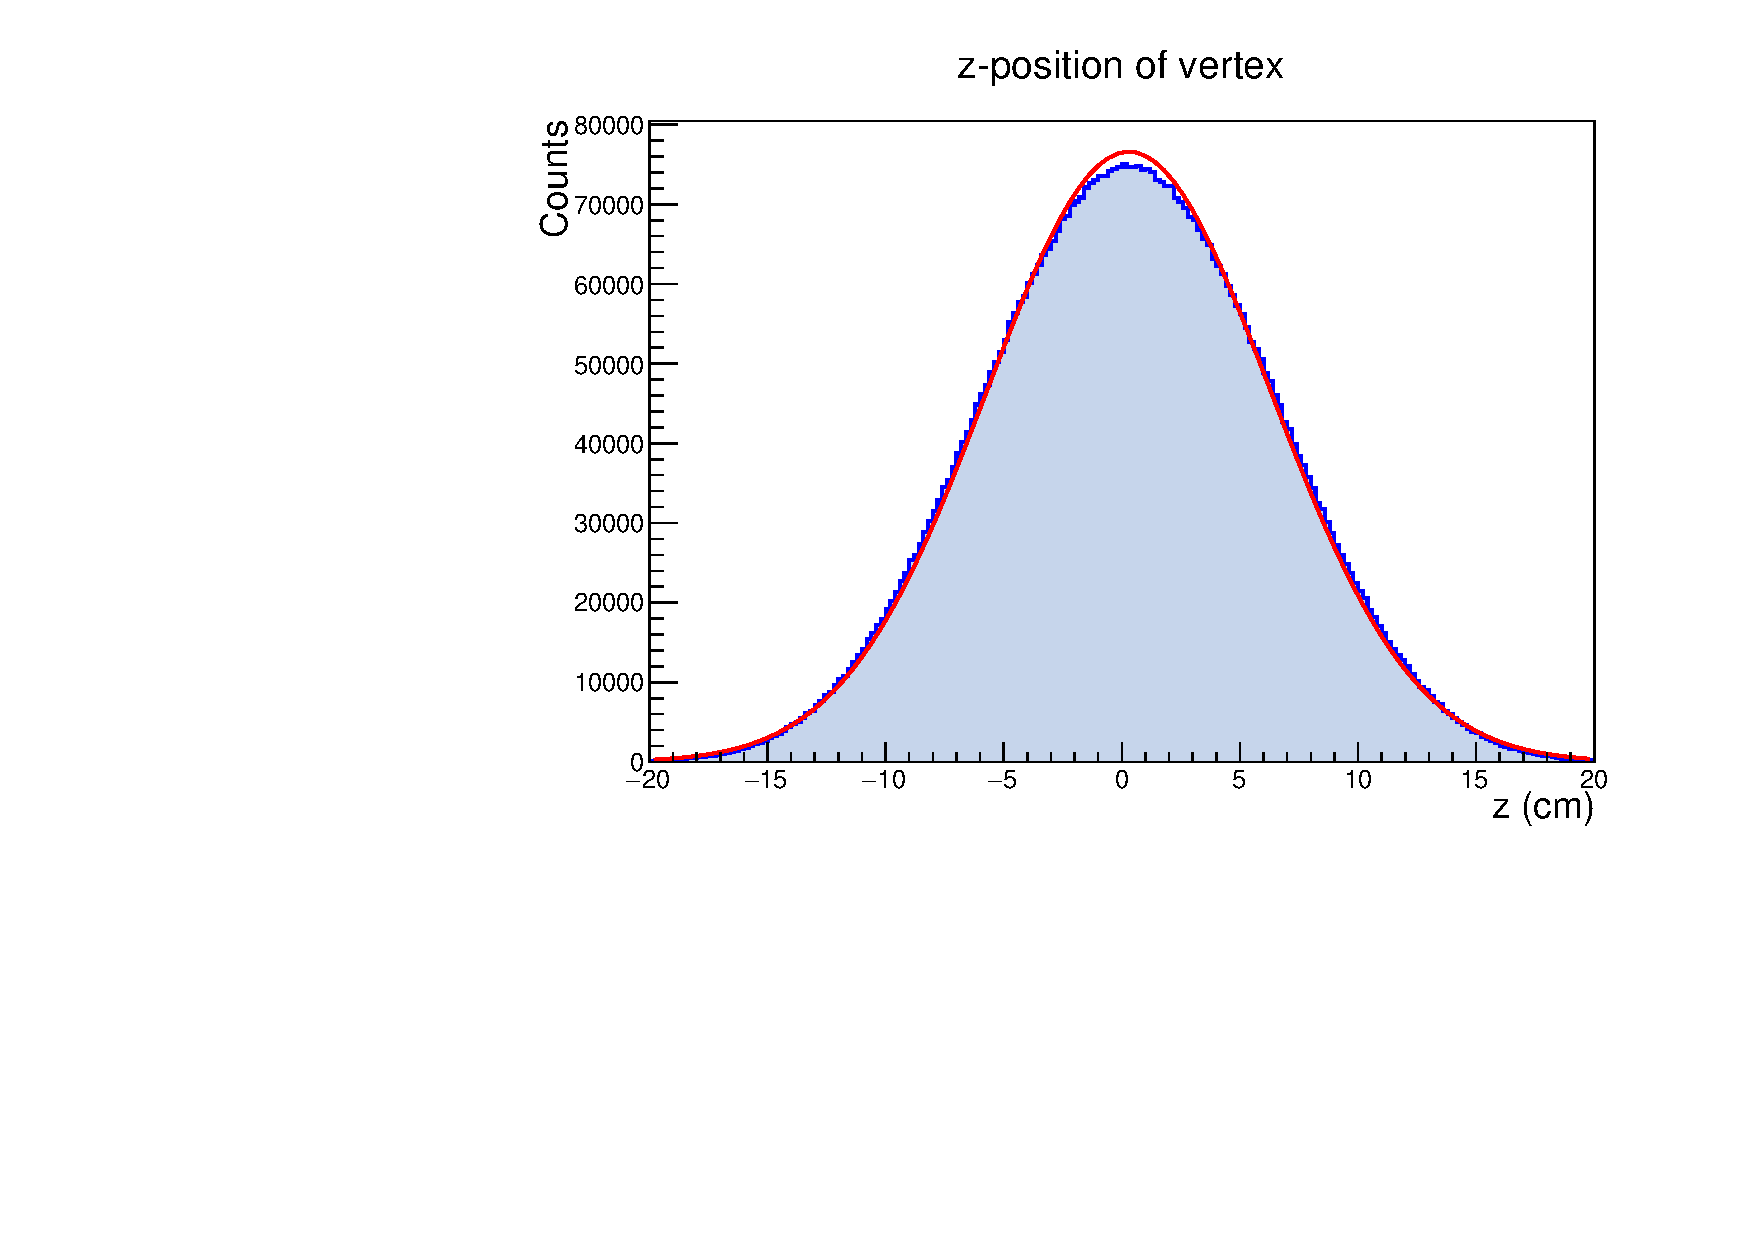
\includegraphics[width=0.95\textwidth]{Plots/pass4_TracksIU/Z.pdf}
                \end{center}
            \end{figure}
        \end{column}
    \end{columns}

\end{frame}

\begin{frame}
    \frametitle{$\eta$-$\varphi$ in the ITS (pass 4, hasITS)}
        \begin{figure}
            \begin{center}
                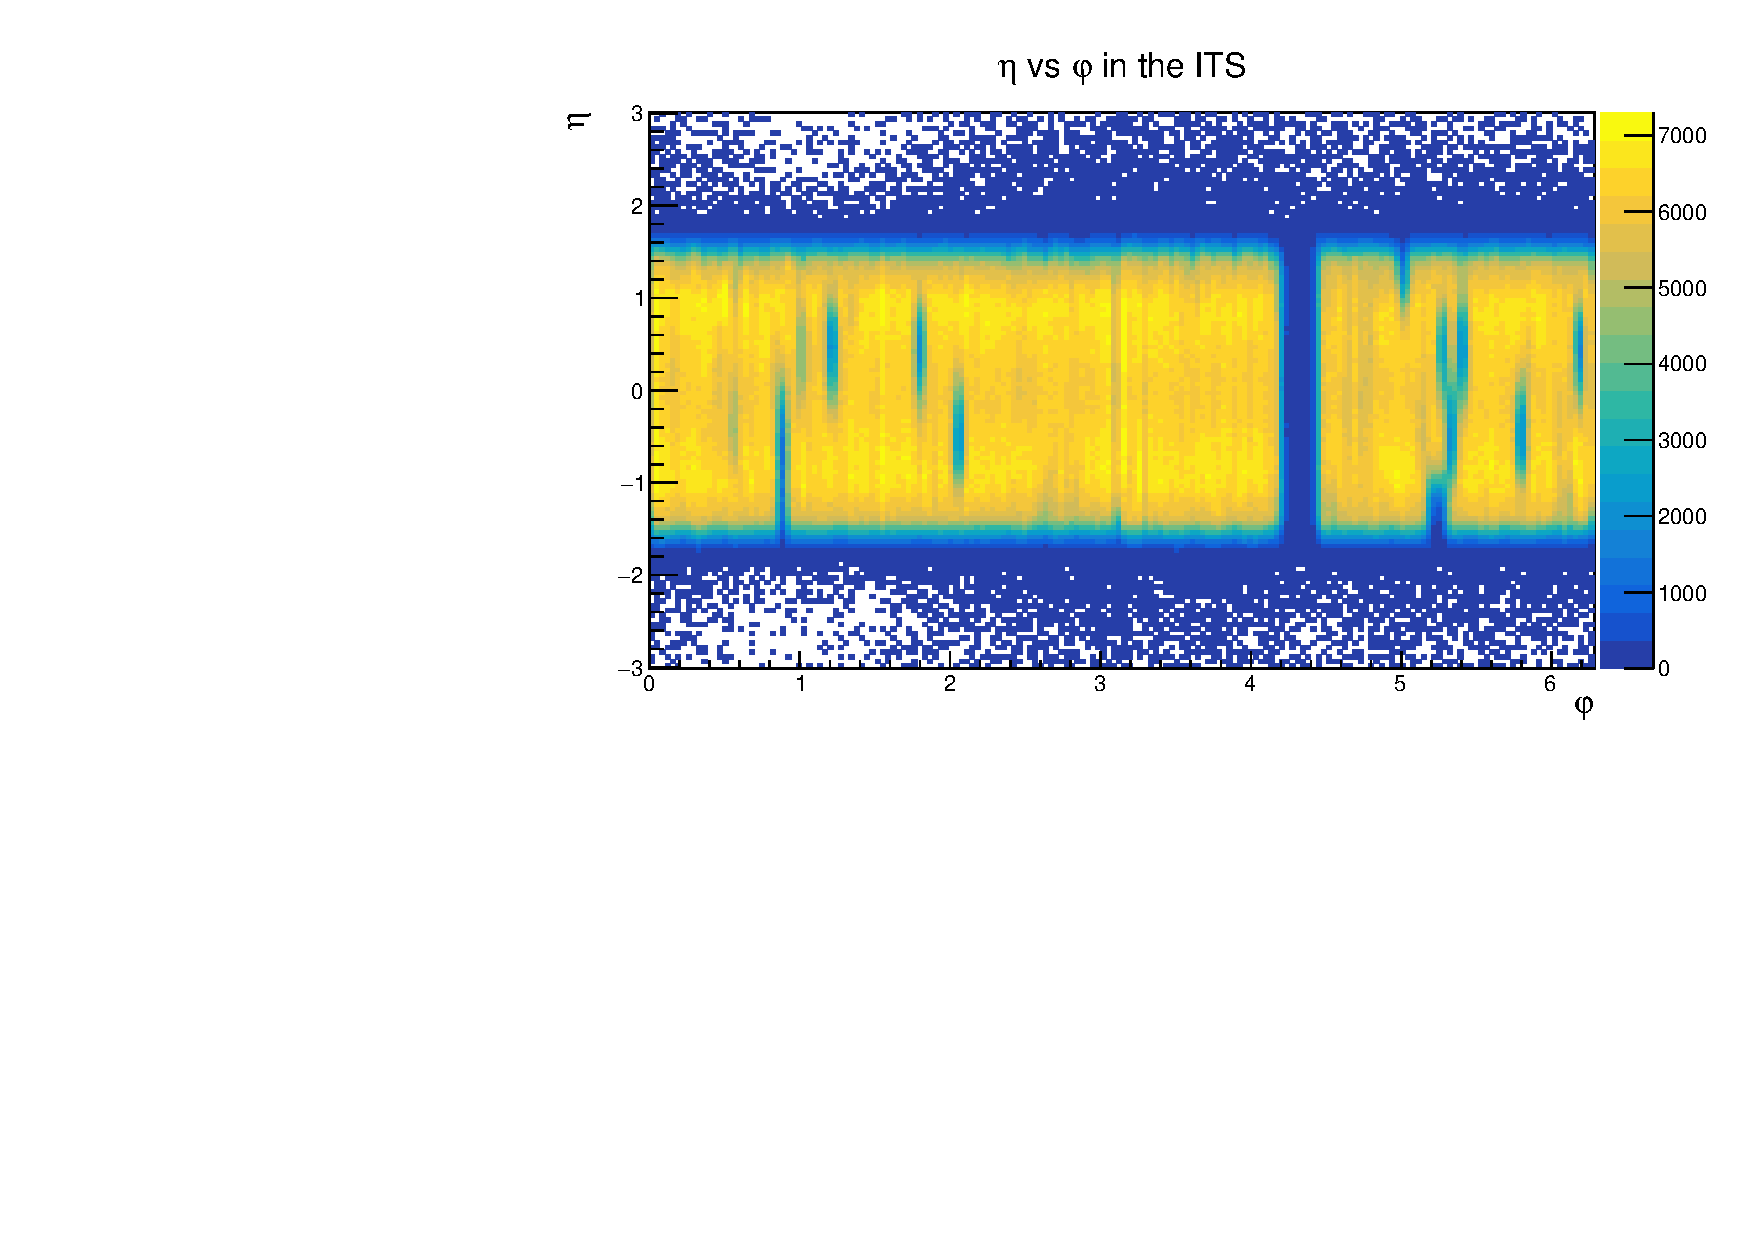
\includegraphics[width=\textwidth]{Plots/pass4_TracksIU/eta_phi.pdf}
            \end{center}
        \end{figure}
\end{frame}


\section{Conclusion}

\begin{frame}
    \frametitle{Conclusion}

    \begin{itemize}
        \item Doing this fairly basic analysis is not what O2 was made for, so it is often hard to access the variables we want to use
        \item The documentation is also not made for it, so working out what these variables mean is hard, if not impossible
        \item If this is going to be studied more, it requires either additions to O2 or analysis at a deeper level, before the AOD's get made
    \end{itemize}

\end{frame}

\begin{frame}
    \begin{center}
        {\Huge Thank you!}
    \end{center}

\end{frame}

%%%%%%%%%%%%%%%%%%%%%%%%%%%%%%%%%%%%%%%%%%%%%%%%%%%%%%%%%%%%%%%%%%%%%%%%%%%%%%%%%

\section{Backup}

\begin{frame}
    \frametitle{MFT Kinematics (pass 4)}

    \begin{columns}
        \begin{column}{0.5\textwidth}
            \vspace*{-0.43cm}
            \begin{figure}
                \begin{center}
                    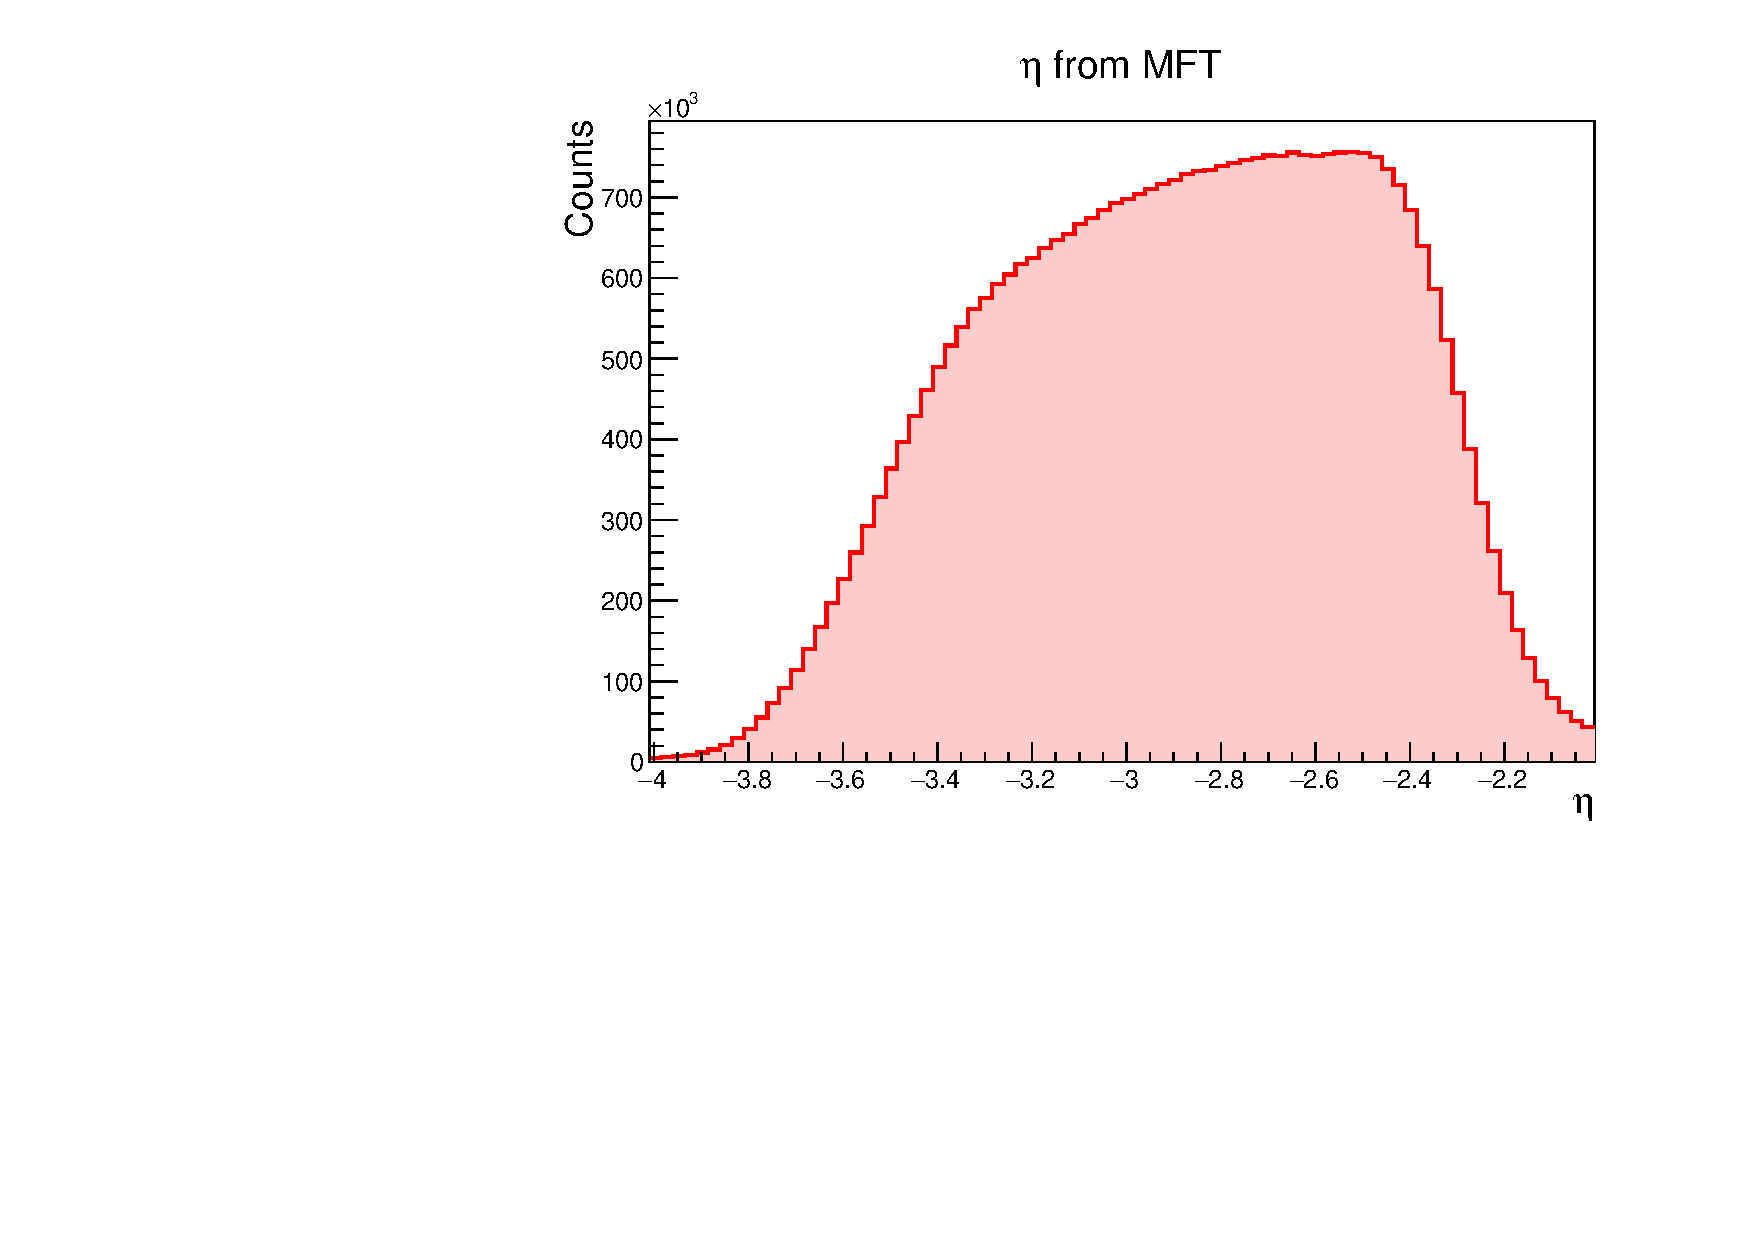
\includegraphics[width=0.95\textwidth]{Plots/pass4_MFT/MFTeta_pass4.pdf}
                \end{center}
            \end{figure}
            \vspace*{-0.6cm}
            \begin{figure}
                \begin{center}
                    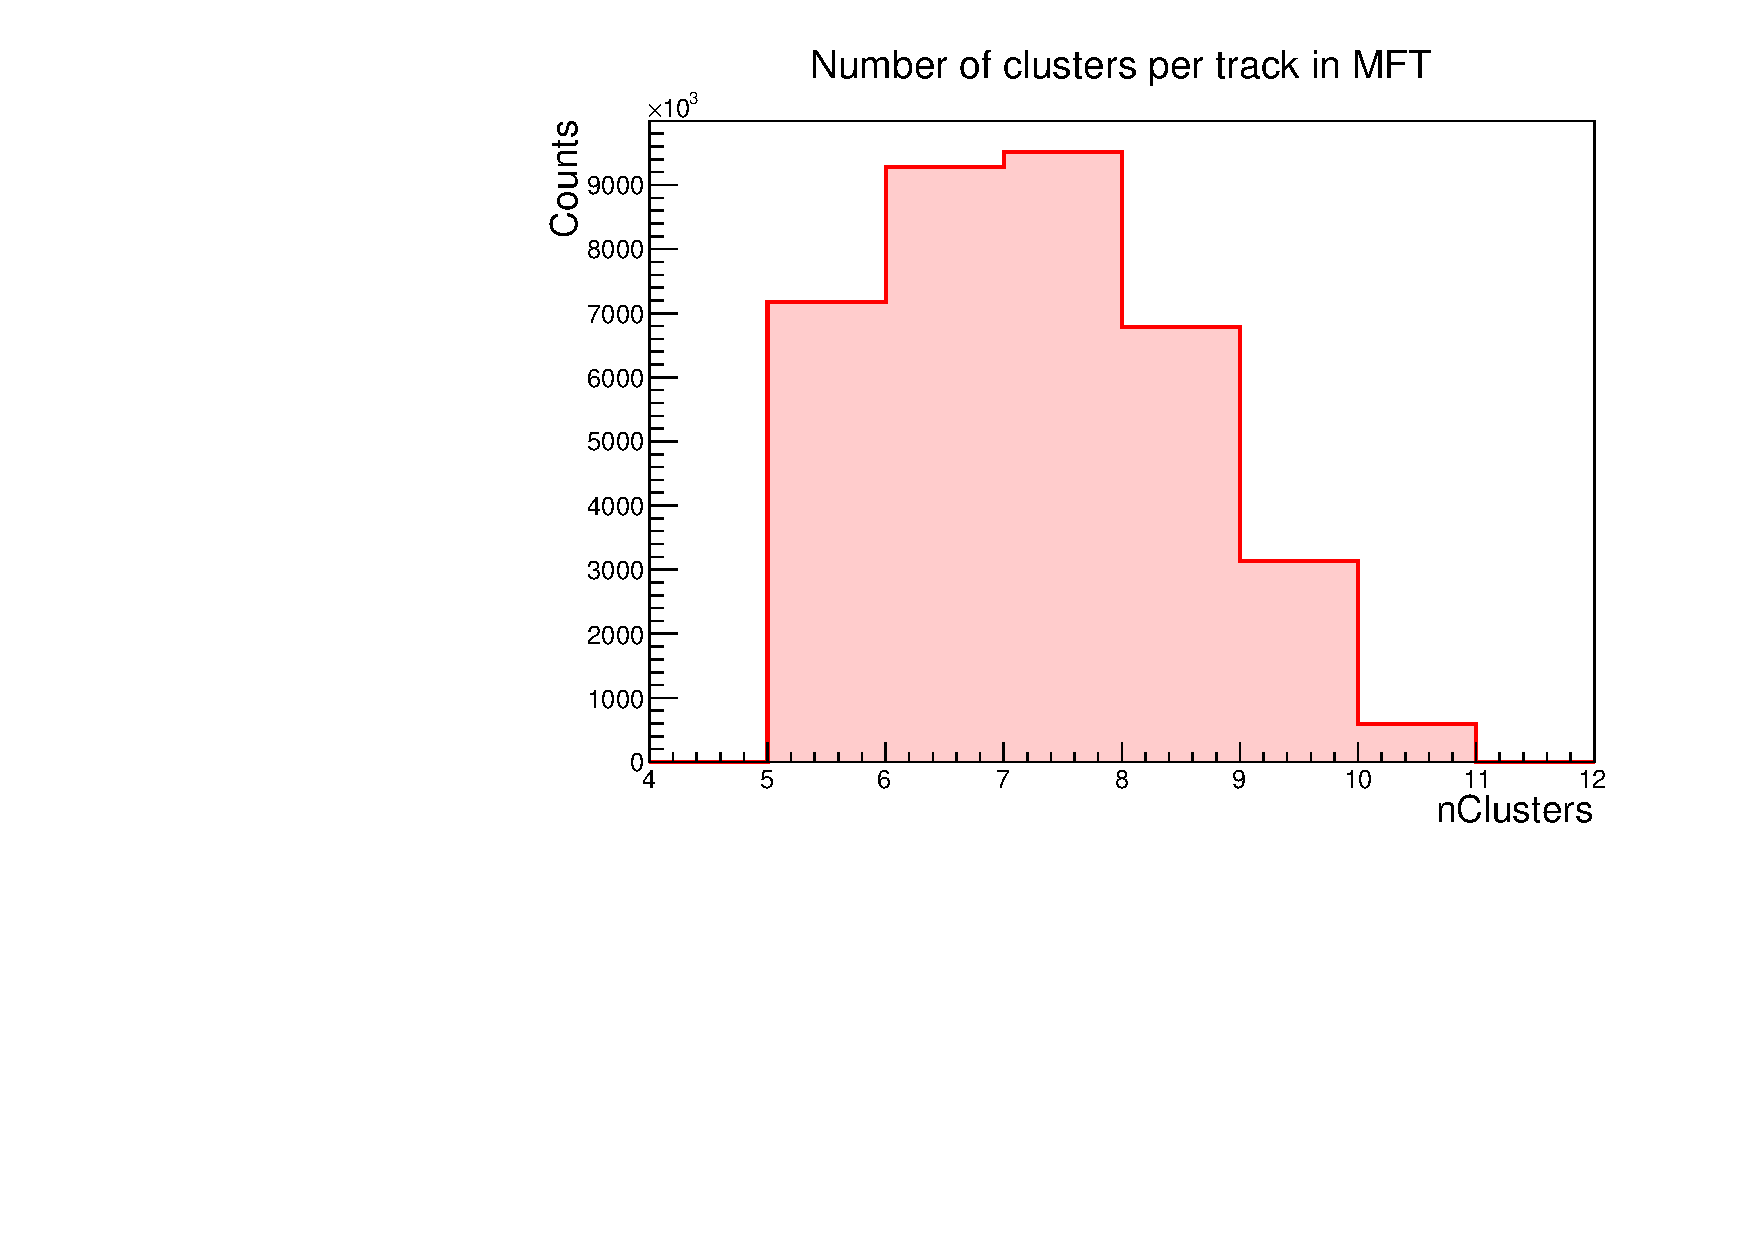
\includegraphics[width=0.95\textwidth]{Plots/pass4_MFT/nClusters_pass4.pdf}
                \end{center}
            \end{figure}
        \end{column}
        \begin{column}{0.5\textwidth}
            \vspace*{-0.43cm}
            \begin{figure}
                \begin{center}
                    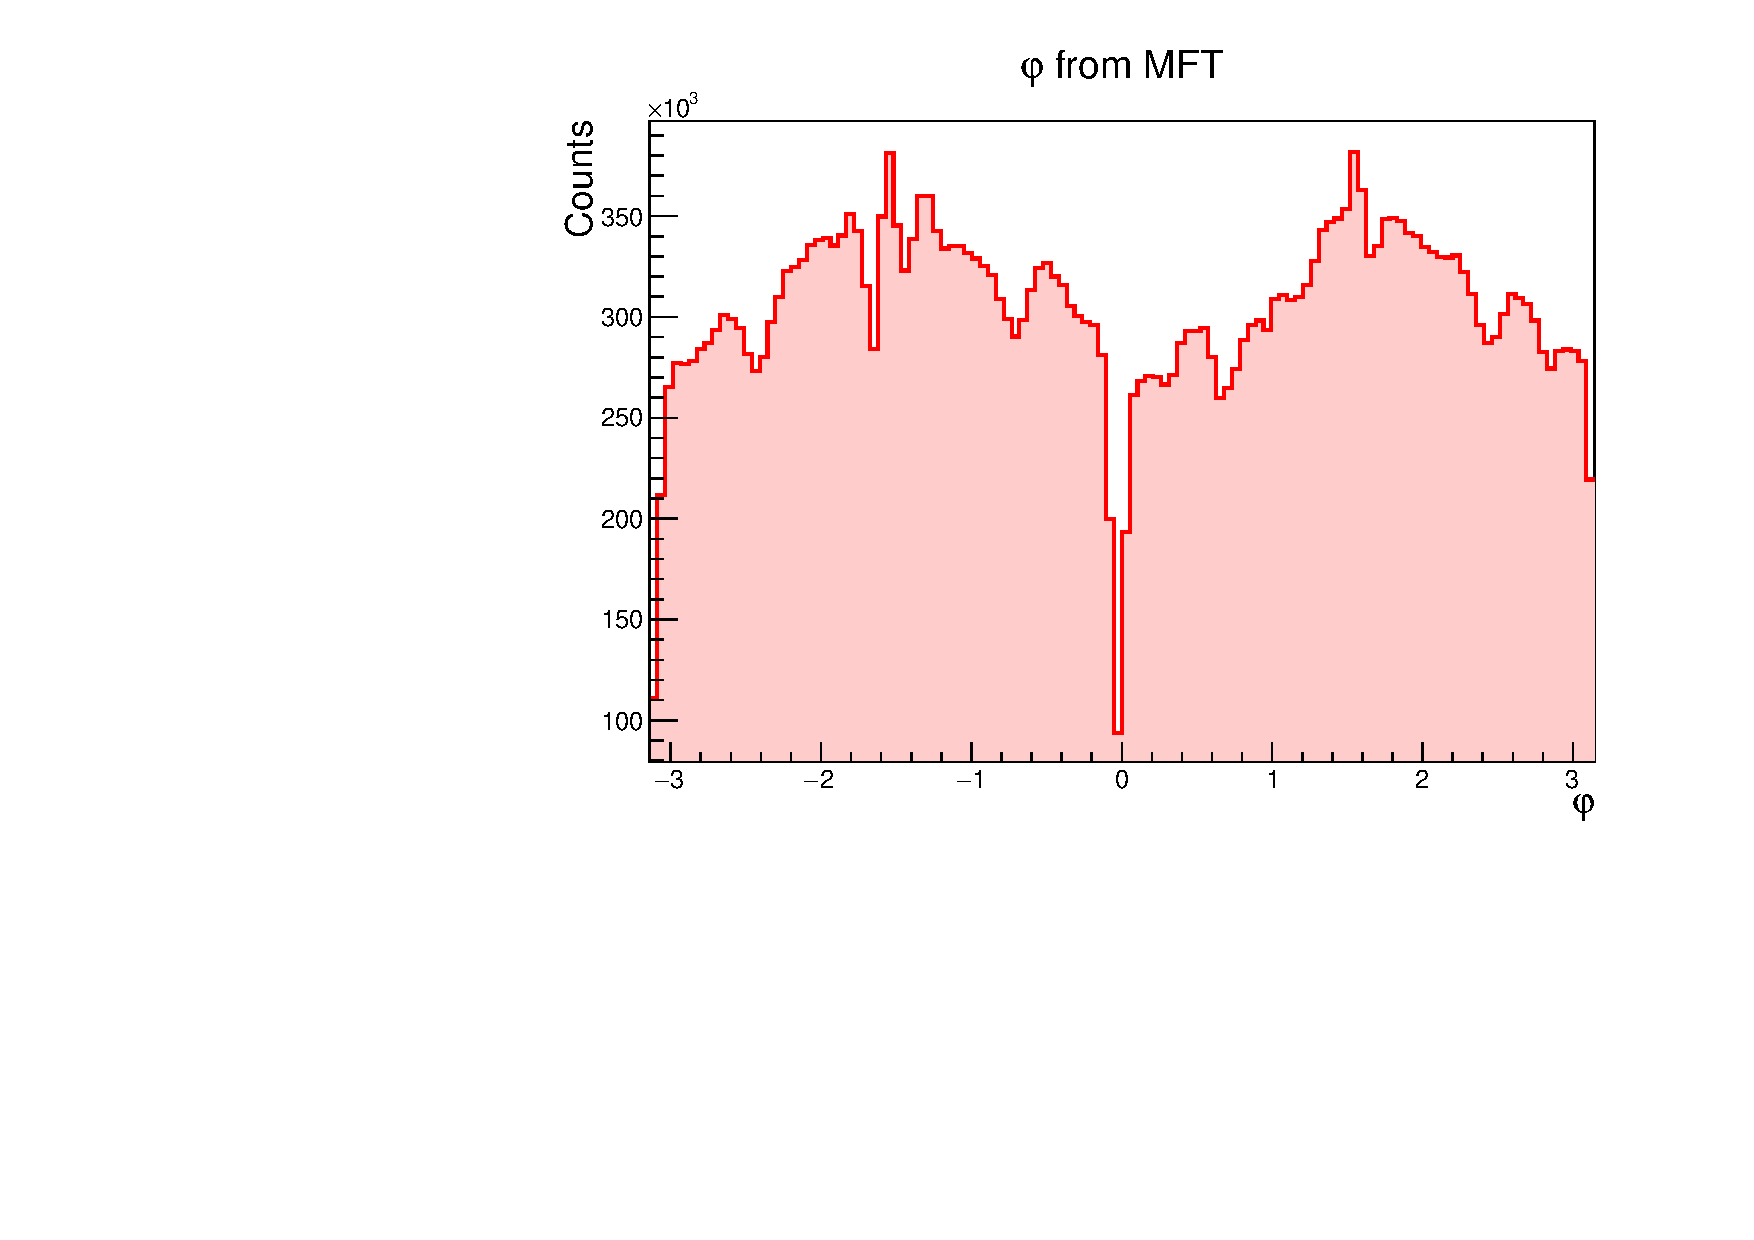
\includegraphics[width=0.95\textwidth]{Plots/pass4_MFT/phi_pass4.pdf}
                \end{center}
            \end{figure}
            \vspace*{-0.6cm}
            \begin{figure}
                \begin{center}
                    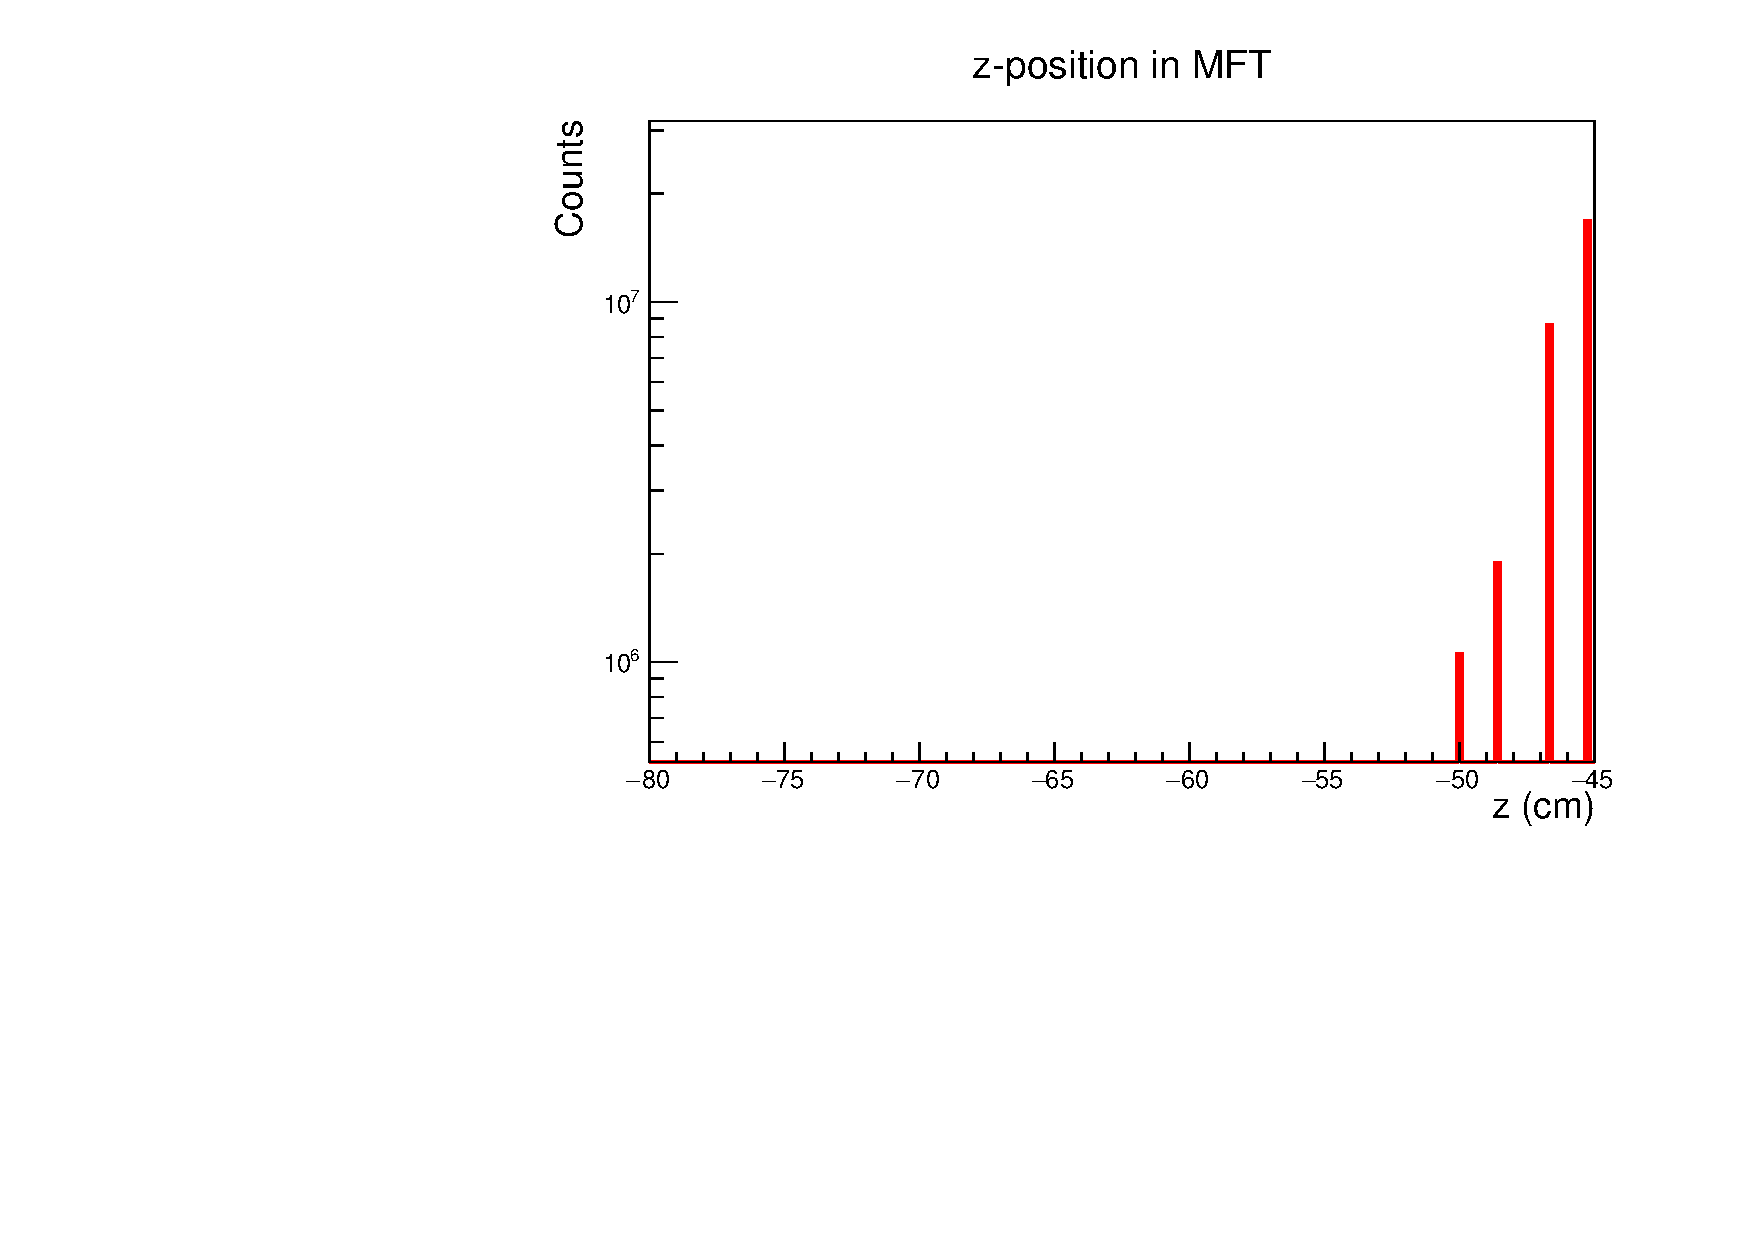
\includegraphics[width=0.95\textwidth]{Plots/pass4_MFT/Z_MFT_pass4.pdf}
                \end{center}
            \end{figure}
        \end{column}
    \end{columns}

\end{frame}

\begin{frame}
    \frametitle{MFT x-y Plots (pass 4)}

    \begin{columns}[T]
        \begin{column}{0.5\textwidth}
            \vspace*{-0.5cm}
            \begin{figure}
                \begin{center}
                    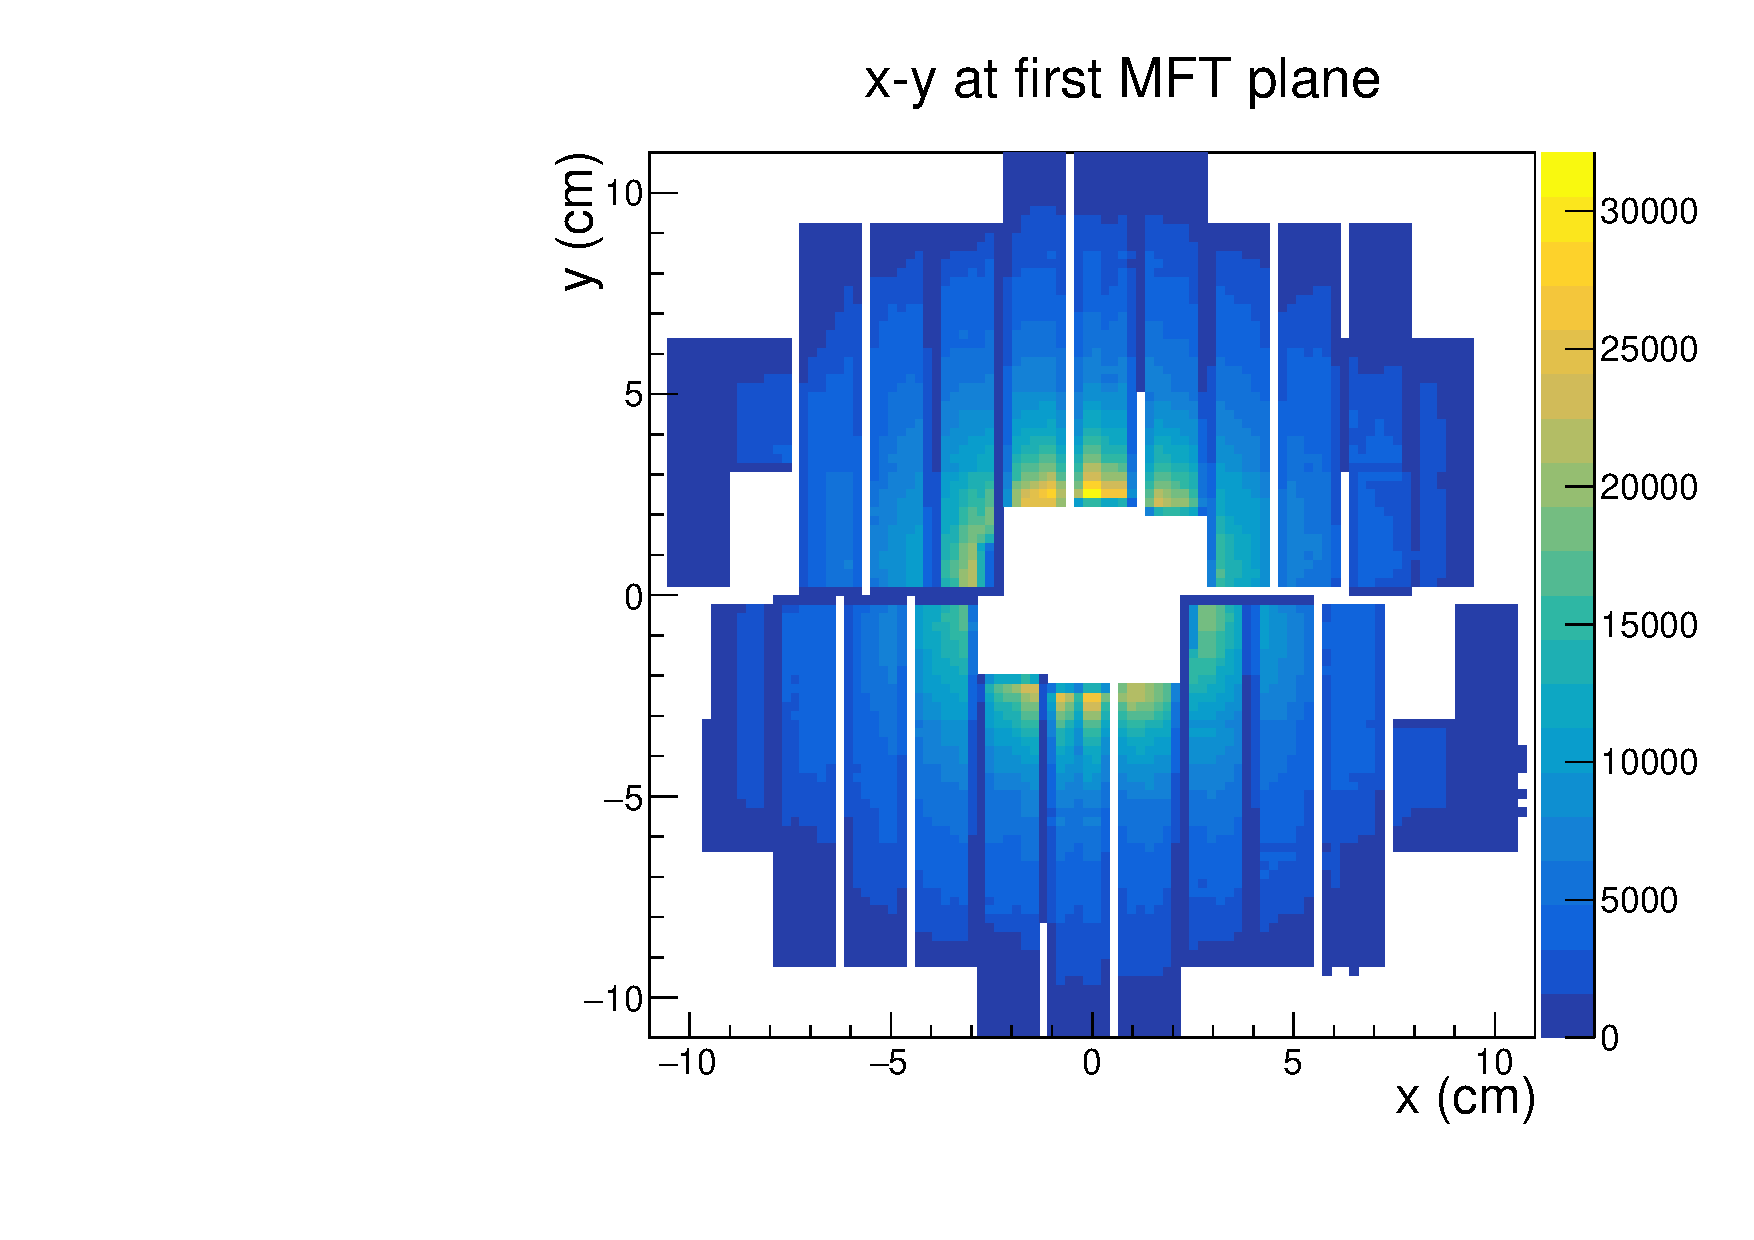
\includegraphics[width=0.7\textwidth]{Plots/pass4_MFT/x_y_1_pass4.pdf}
                \end{center}
            \end{figure}
            \vspace*{-0.7cm}
            \begin{figure}
                \begin{center}
                    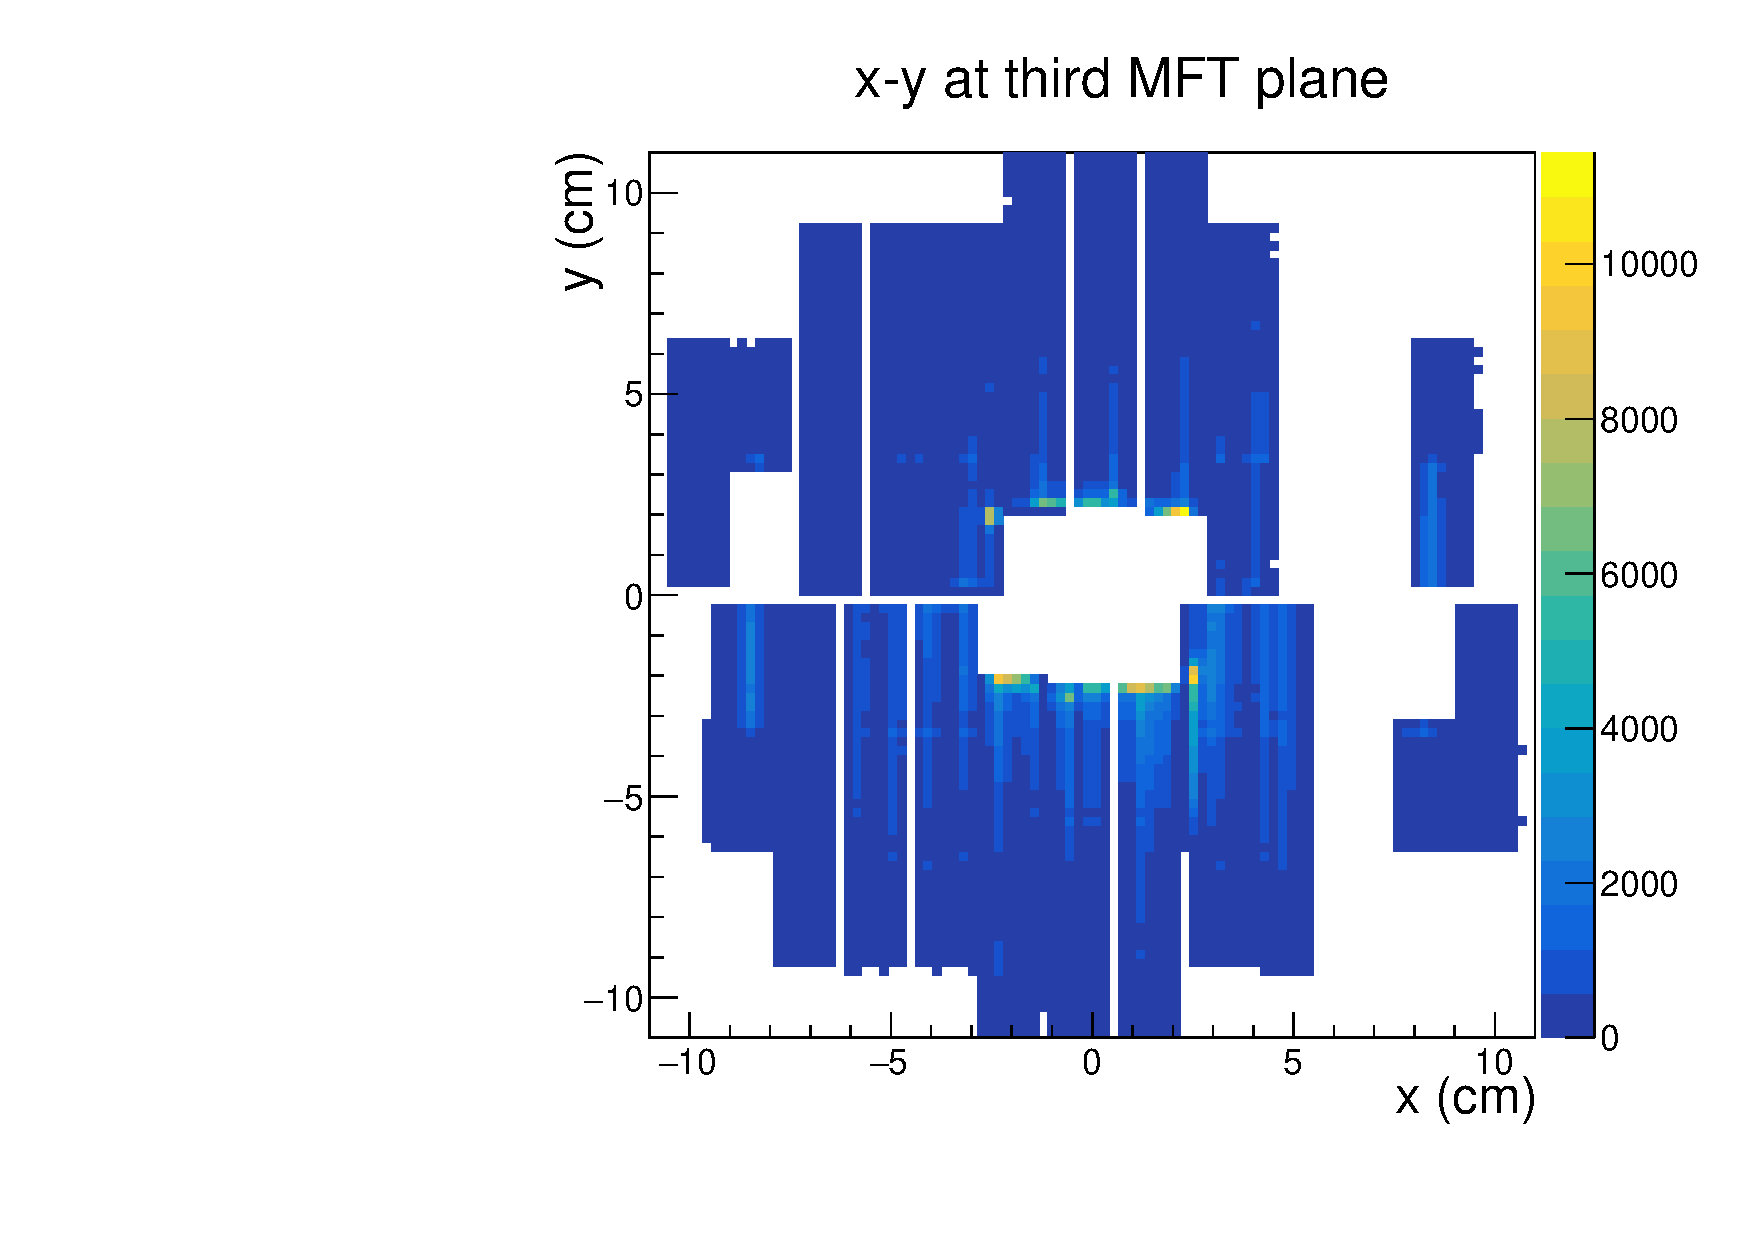
\includegraphics[width=0.7\textwidth]{Plots/pass4_MFT/x_y_3_pass4.pdf}
                \end{center}
            \end{figure}
        \end{column}
        \begin{column}{0.5\textwidth}
            \vspace*{-0.5cm}
            \begin{figure}
                \begin{center}
                    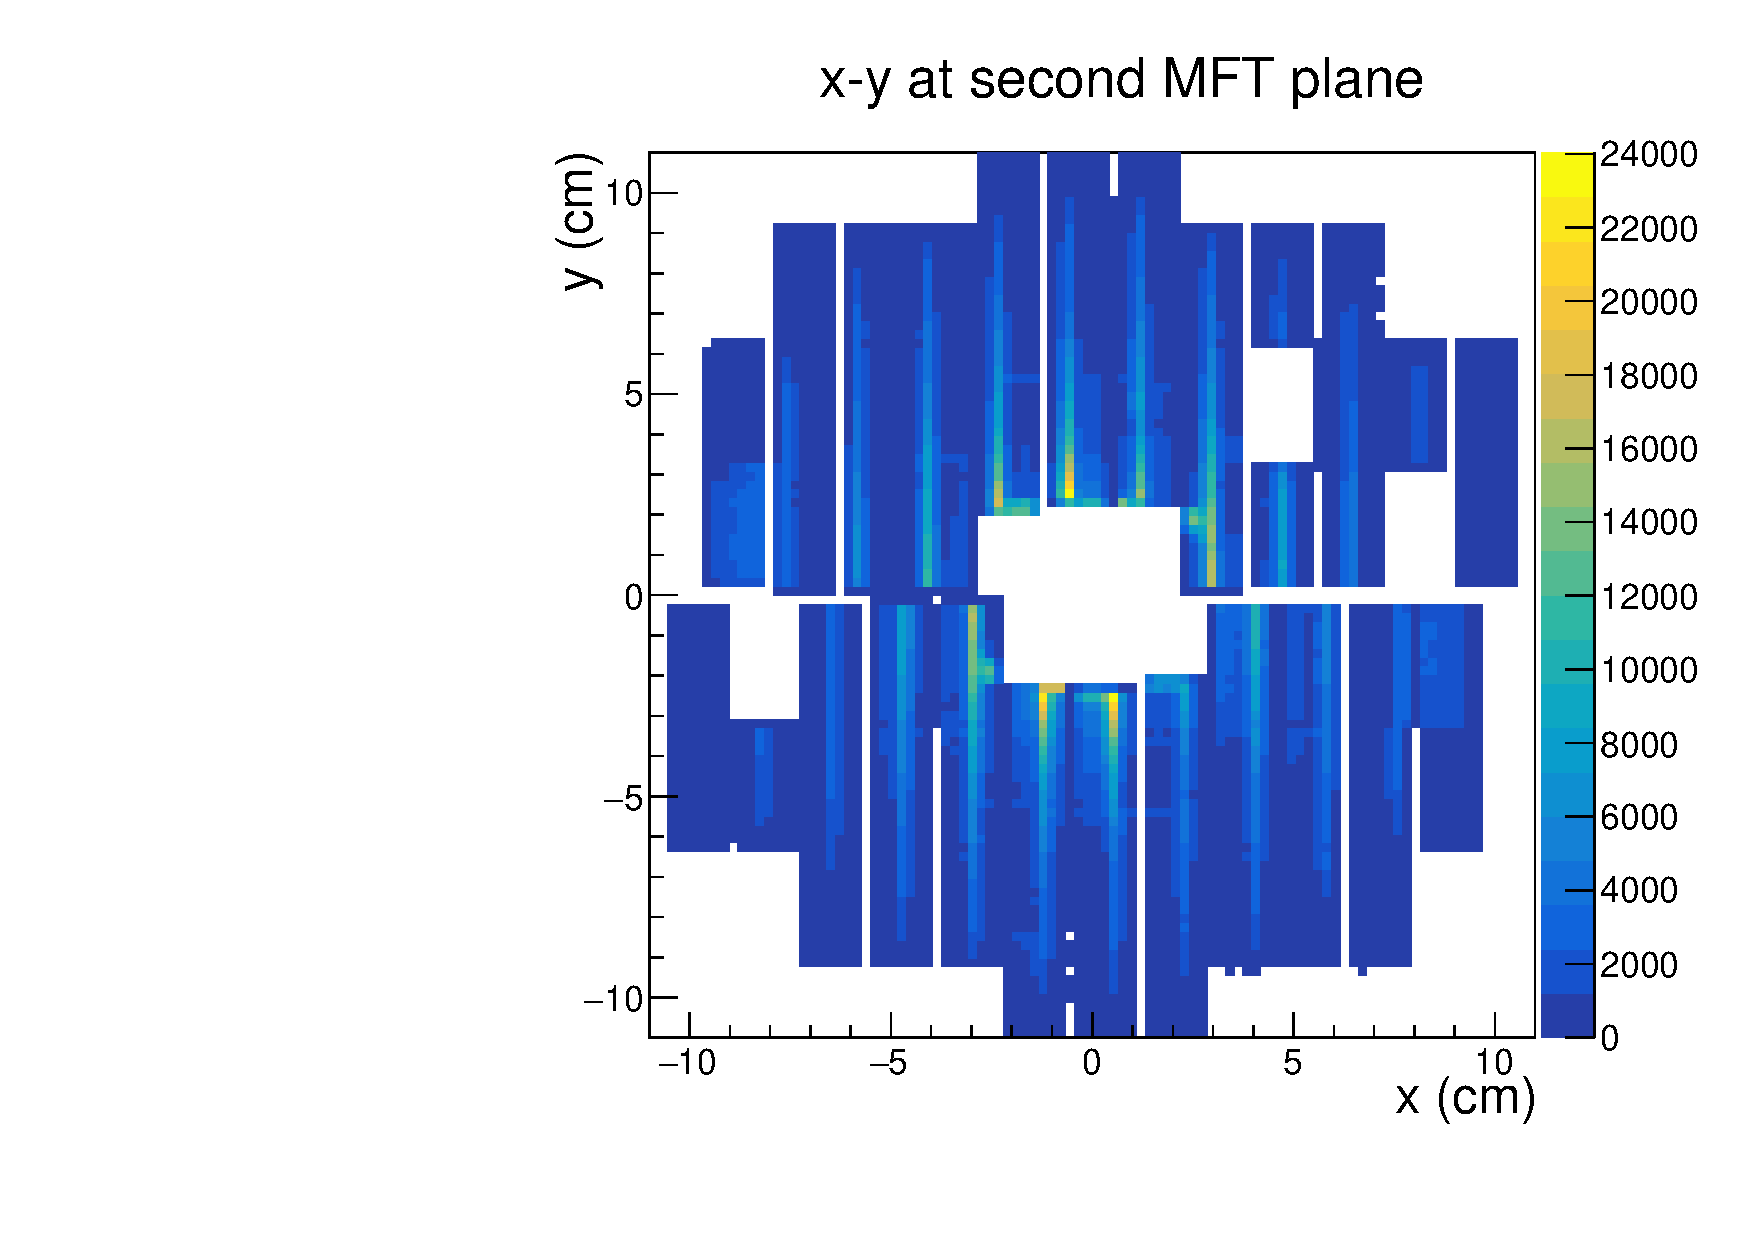
\includegraphics[width=0.7\textwidth]{Plots/pass4_MFT/x_y_2_pass4.pdf}
                \end{center}
            \end{figure}
            \vspace*{-0.7cm}
            \begin{figure}
                \begin{center}
                    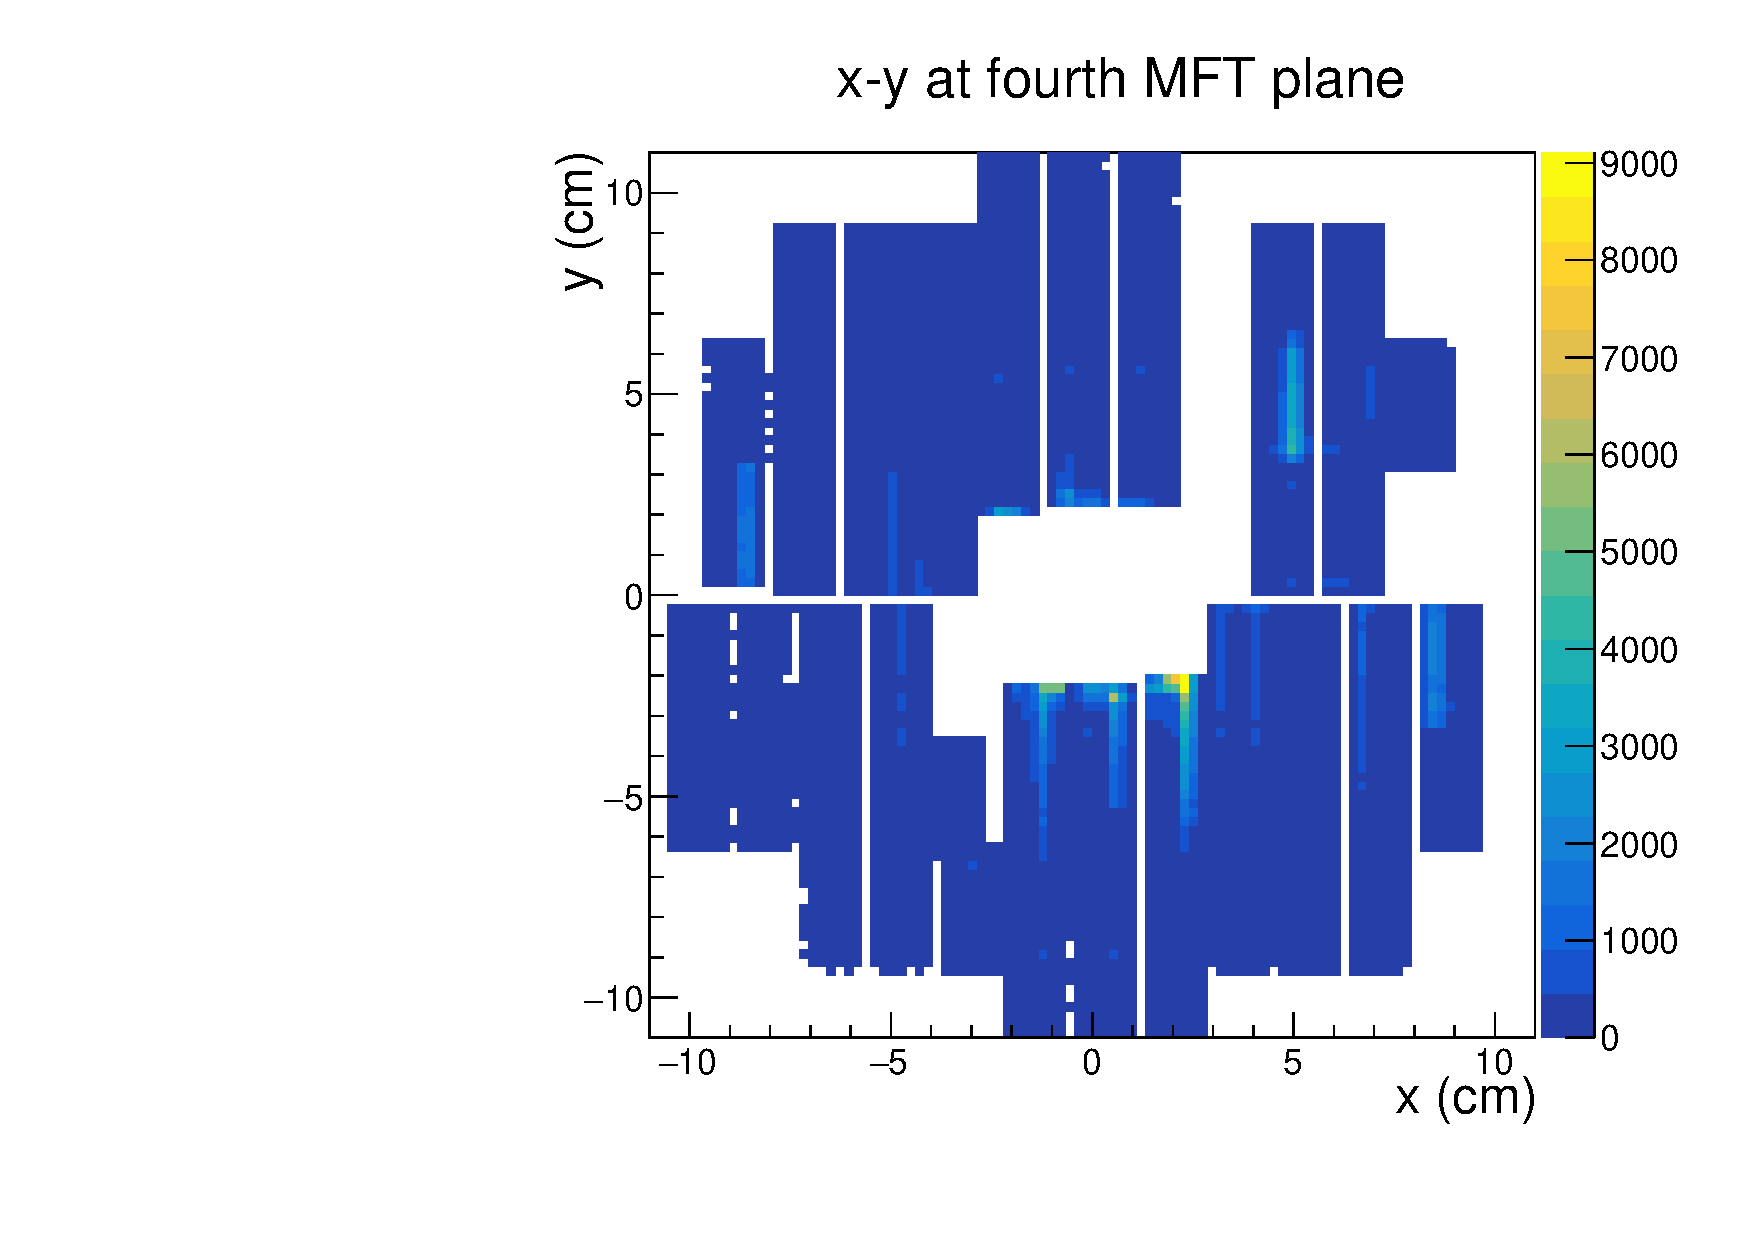
\includegraphics[width=0.7\textwidth]{Plots/pass4_MFT/x_y_4_pass4.pdf}
                \end{center}
            \end{figure}
        \end{column}
    \end{columns}

\end{frame}

\begin{frame}
    \frametitle{$\eta$-$\varphi$ in the MFT (pass 4)}
        \begin{figure}
            \begin{center}
                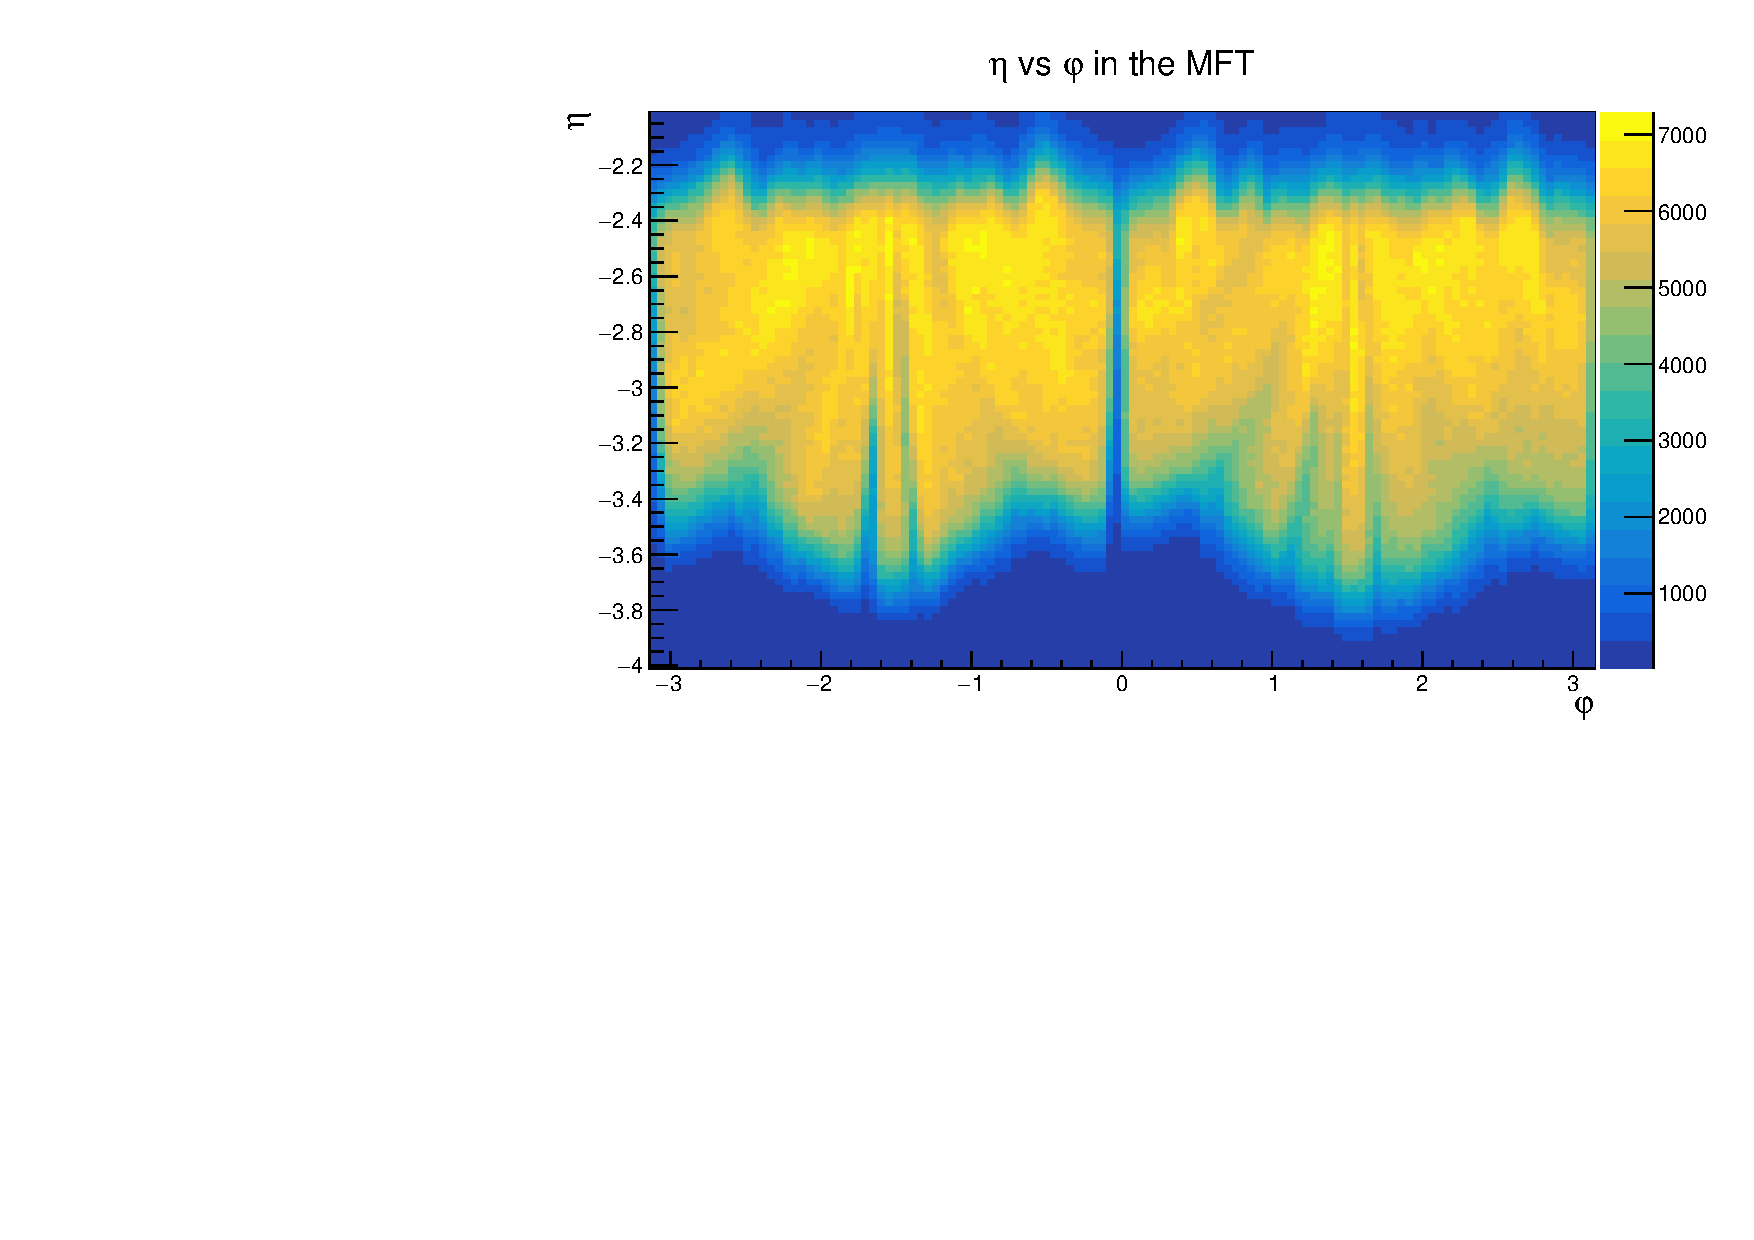
\includegraphics[width=0.9\textwidth]{Plots/pass4_MFT/eta_phi_pass4.pdf}
            \end{center}
        \end{figure}
\end{frame}

\begin{frame}
    \frametitle{ITS Kinematics (pass 4)}

    \begin{columns}
        \begin{column}{0.5\textwidth}
            \vspace*{-0.43cm}
            \begin{figure}
                \begin{center}
                    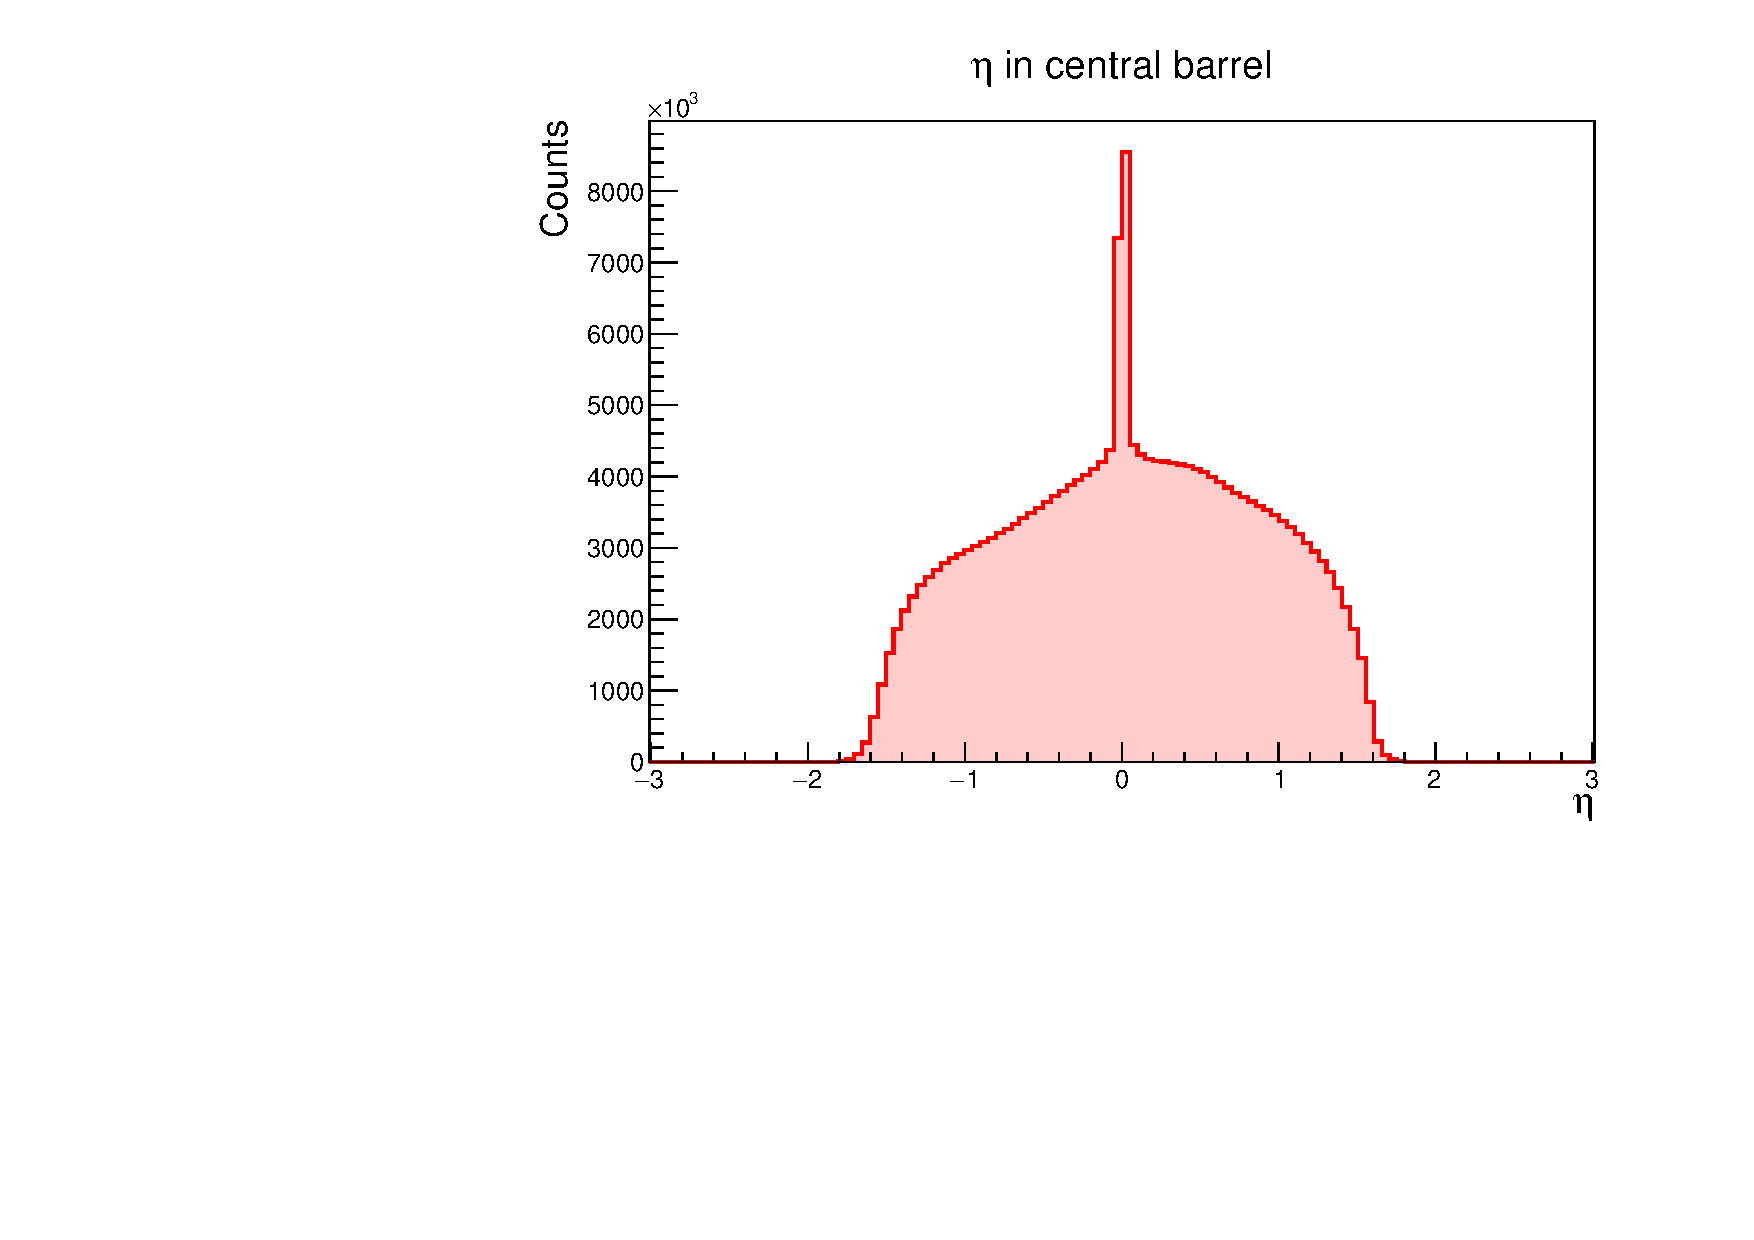
\includegraphics[width=0.95\textwidth]{Plots/pass4_TracksIU_nohasITS/eta.pdf}
                \end{center}
            \end{figure}
            \vspace*{-0.6cm}
            \begin{figure}
                \begin{center}
                    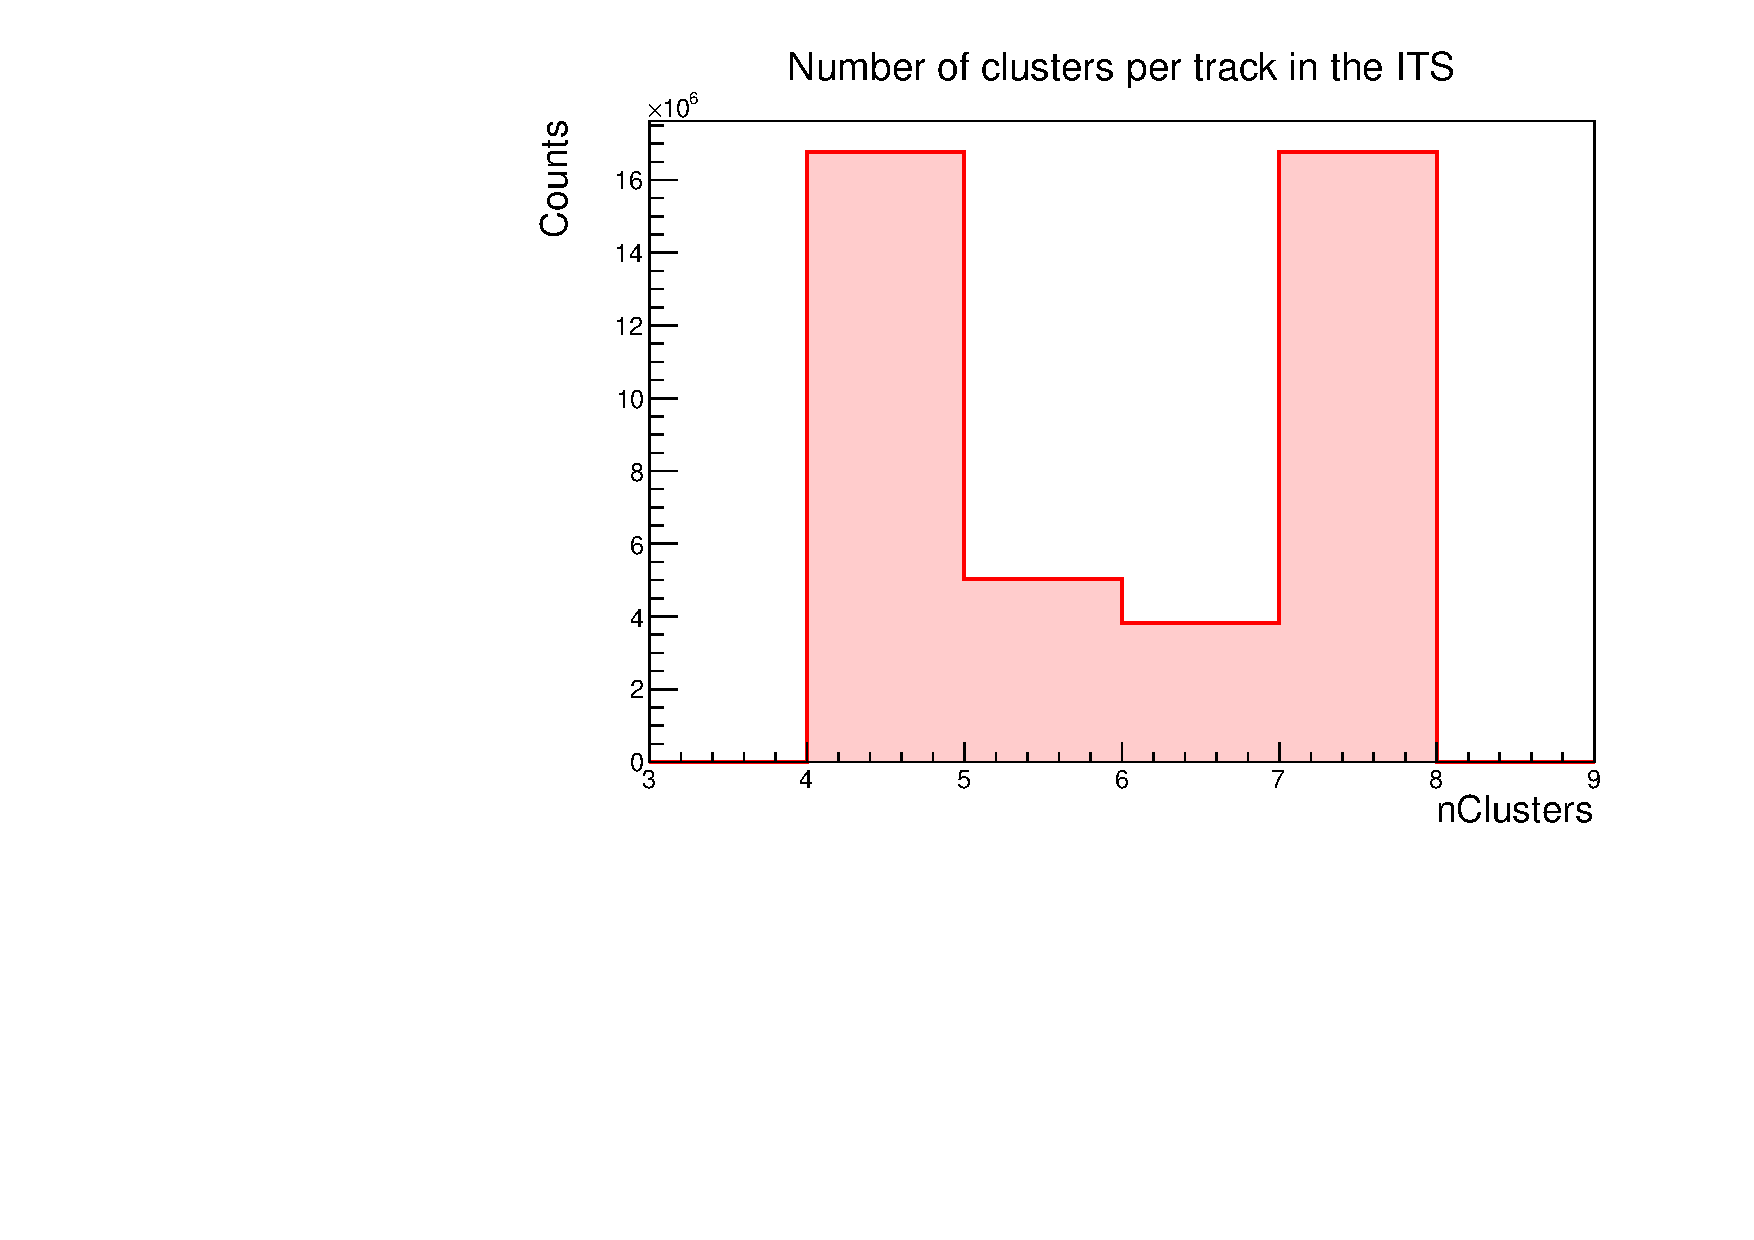
\includegraphics[width=0.95\textwidth]{Plots/pass4_TracksIU_nohasITS/itsNCls.pdf}
                \end{center}
            \end{figure}
        \end{column}
        \begin{column}{0.5\textwidth}
            \vspace*{-0.43cm}
            \begin{figure}
                \begin{center}
                    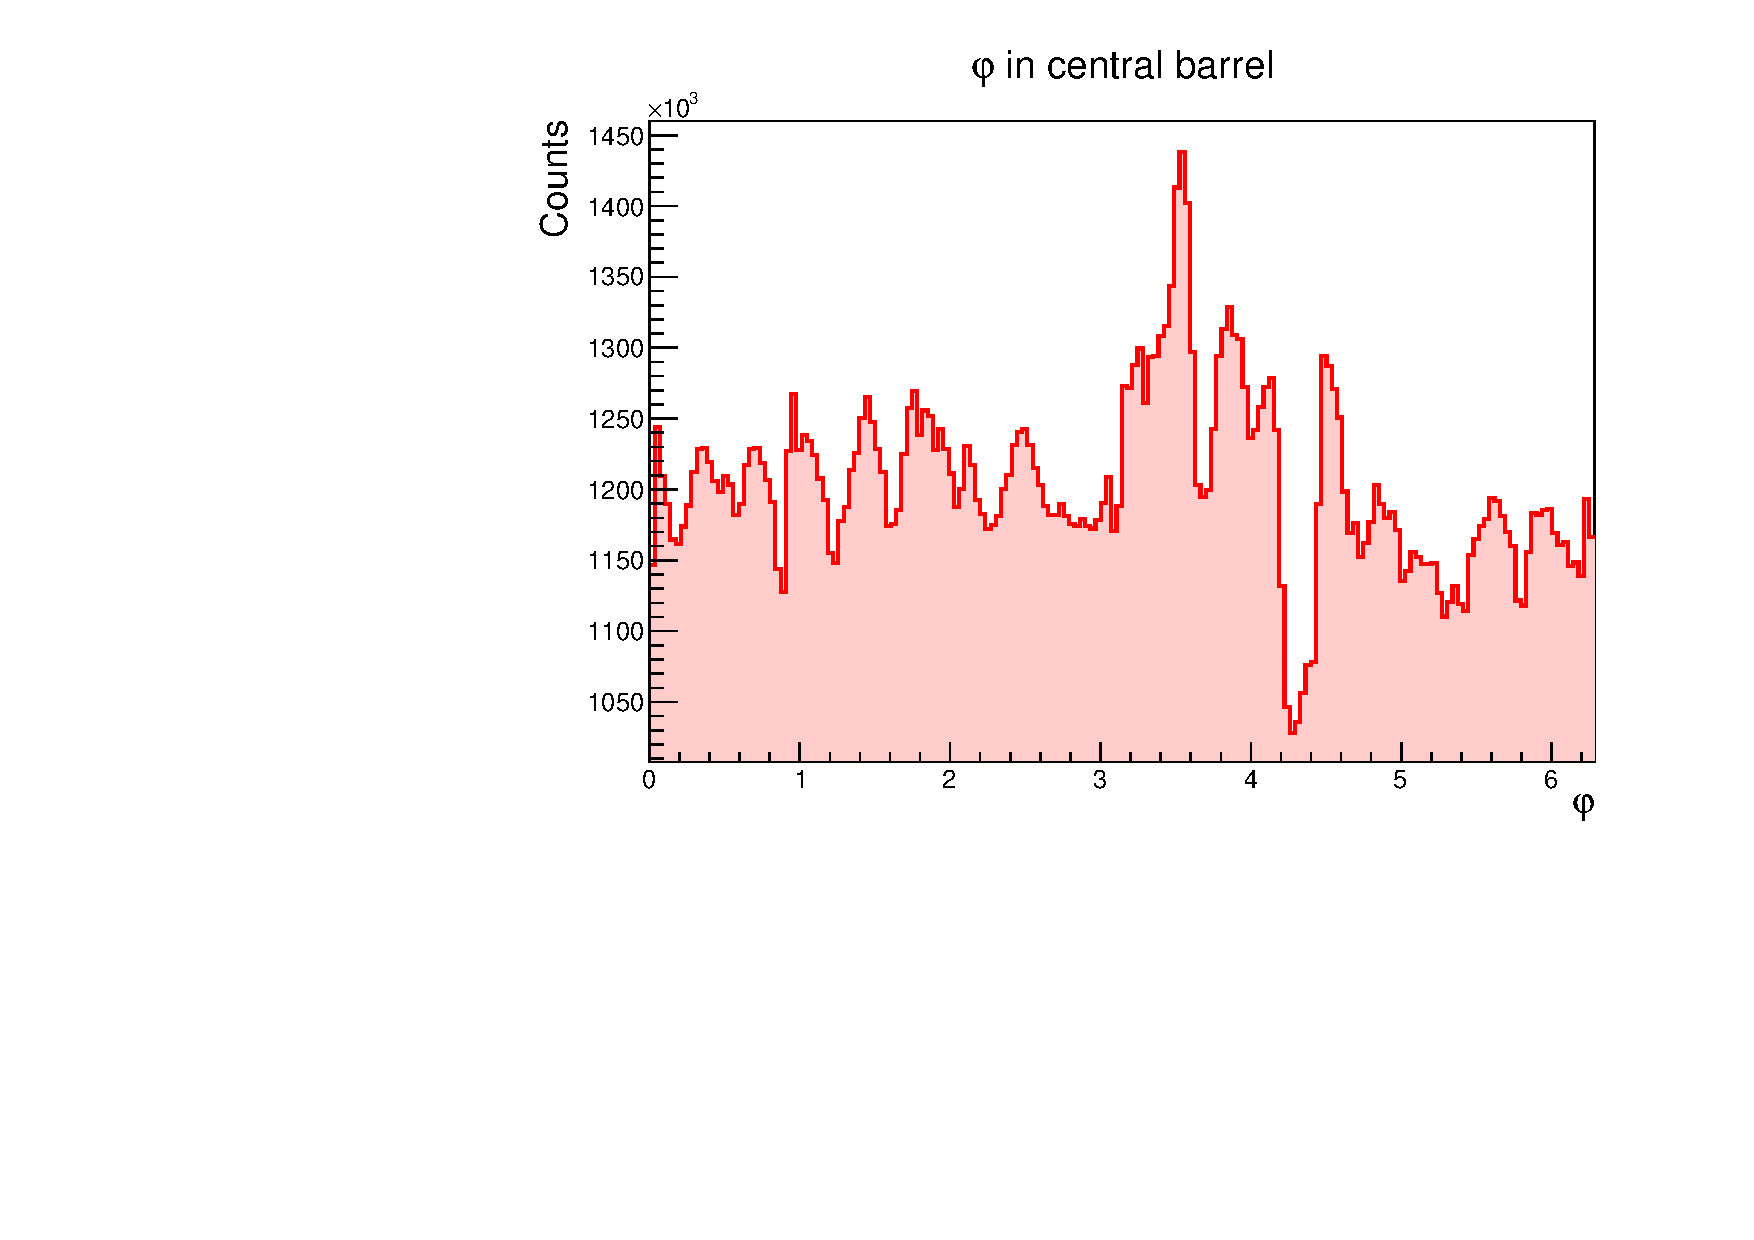
\includegraphics[width=0.95\textwidth]{Plots/pass4_TracksIU_nohasITS/phi.pdf}
                \end{center}
            \end{figure}
            \vspace*{-0.6cm}
            \begin{figure}
                \begin{center}
                    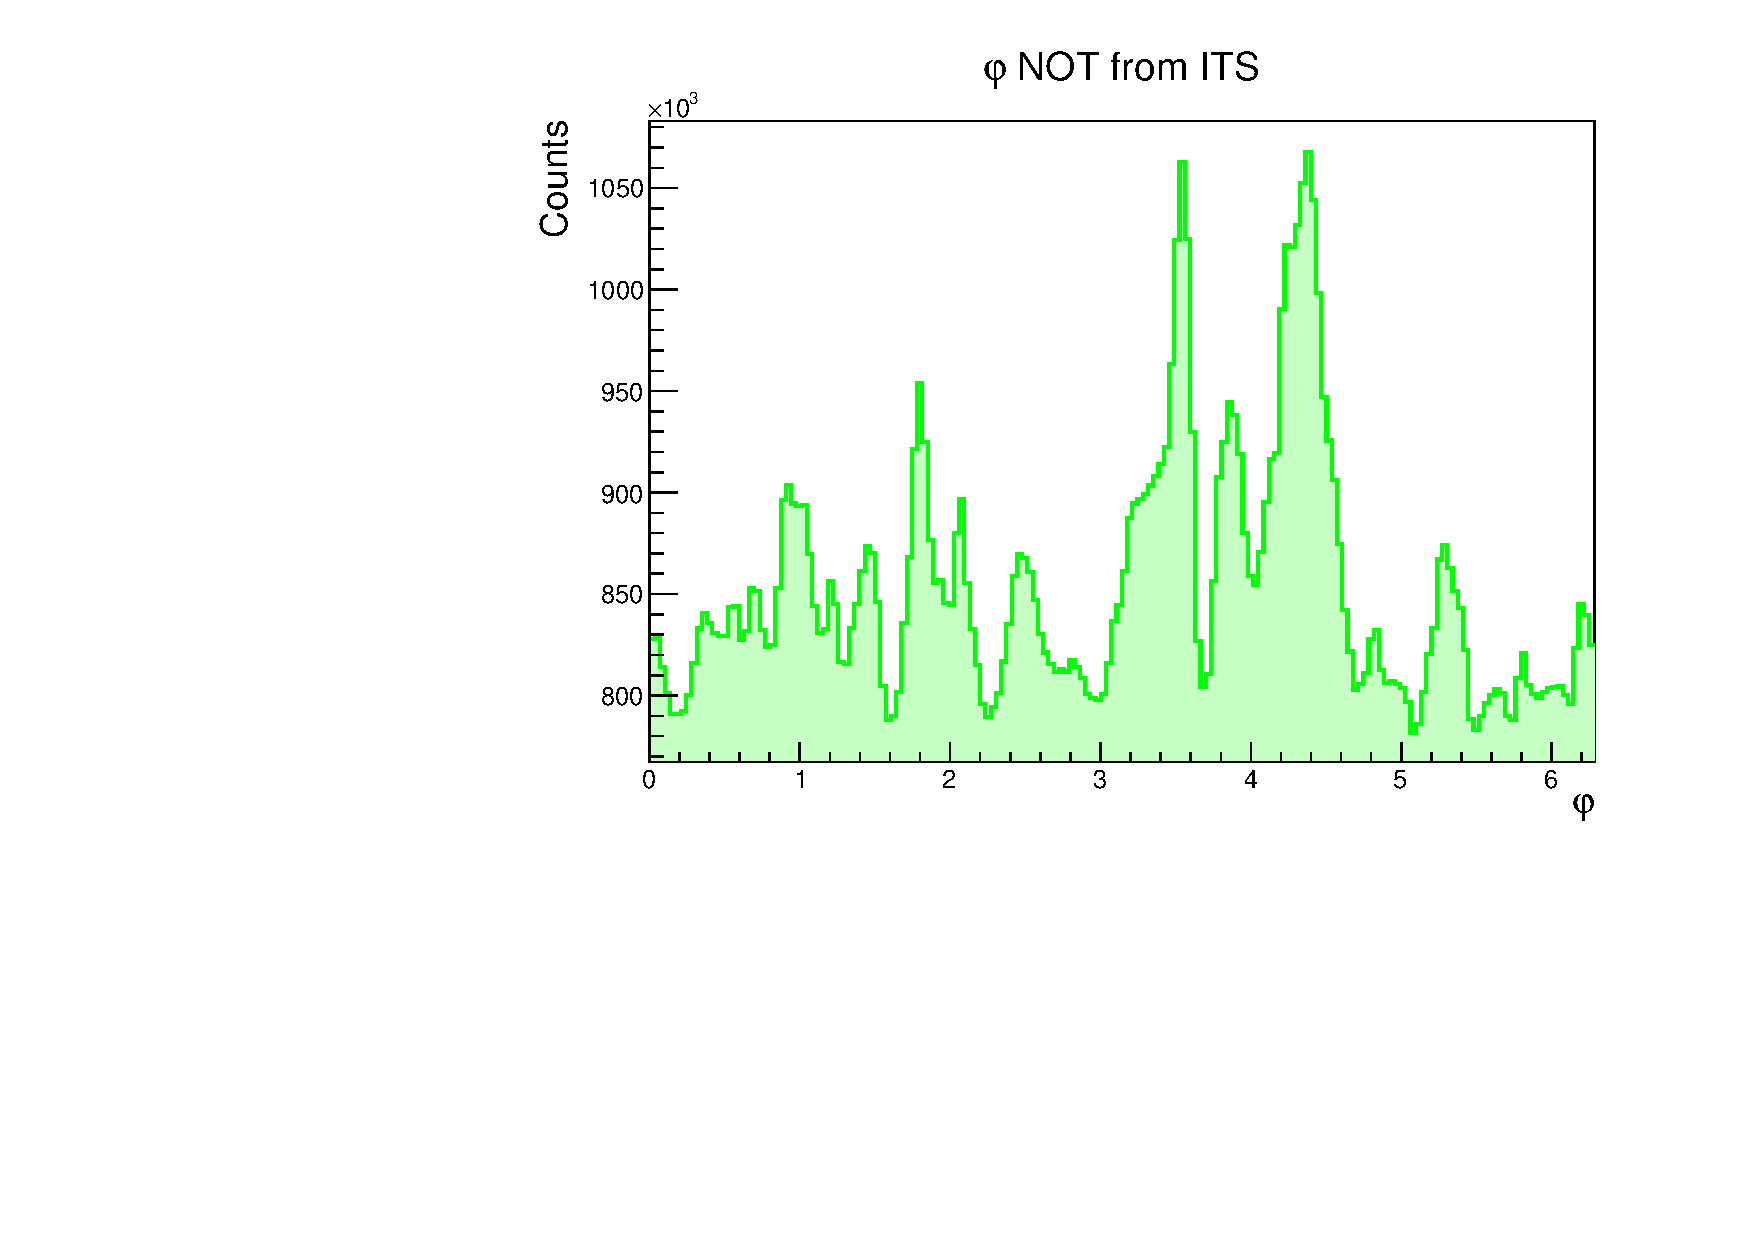
\includegraphics[width=0.95\textwidth]{Plots/phi_no_ITS.pdf}
                \end{center}
            \end{figure}
        \end{column}
    \end{columns}

\end{frame}





\end{document}